% Capitolo 4 - Compliance Integrata e Governance: Ottimizzazione attraverso Sinergie Normative
%\refsection % <--- INIZIA LA SEZIONE DI RIFERIMENTO
\chapter{\texorpdfstring{Compliance Integrata e Governance: Ottimizzazione attraverso Sinergie Normative}{Capitolo 4 - Compliance Integrata e Governance: Ottimizzazione attraverso Sinergie Normative}}
\label{cap4_compliance_integration}

\section{\texorpdfstring{Introduzione: La Conformità Normativa come Vantaggio Competitivo}{4.1 - Introduzione: La Conformità Normativa come Vantaggio Competitivo}}

I capitoli precedenti hanno stabilito come le vulnerabilità architetturali siano la causa principale degli attacchi informatici (Capitolo 2) e come le infrastrutture moderne possano abilitare prestazioni e sicurezza superiori (Capitolo 3). Tuttavia, ogni decisione tecnologica opera all'interno di un panorama normativo complesso che richiede un'analisi approfondita. L'analisi di settore, basata su dati aggregati da 1.847 incidenti nel periodo 2022-2024, mostra che il 68\% delle violazioni di dati sfrutta lacune nella conformità normativa \autocite{verizon2024}. 

Questo capitolo affronta la sfida della conformità multi-standard attraverso un cambio di paradigma fondamentale: la trasformazione della conformità da costo operativo obbligatorio a fattore abilitante di vantaggio competitivo. L'analisi si basa su un approccio quantitativo rigoroso che modella matematicamente le interdipendenze normative tra i tre principali standard del settore (\gls{pci-dss} 4.0, \gls{gdpr}, \gls{nis2}), fornendo evidenze empiriche robuste per la validazione dell'ipotesi H3 della ricerca.

La metodologia adottata combina teoria dei grafi per mappare le relazioni tra requisiti, programmazione lineare per l'ottimizzazione delle risorse, e analisi stocastica per la quantificazione del rischio. Questo approccio multidisciplinare permette di superare i limiti degli approcci tradizionali, tipicamente frammentati e sub-ottimali, offrendo un modello integrato validato su dati reali provenienti da 47 organizzazioni del settore.

\section{\texorpdfstring{Analisi Quantitativa del Panorama Normativo nella Grande Distribuzione}{4.2 - Analisi Quantitativa del Panorama Normativo nella Grande Distribuzione}}

\subsection{\texorpdfstring{Metodologia di Quantificazione degli Impatti Economici}{4.2.1 - Metodologia di Quantificazione degli Impatti Economici}}

L'implementazione del \gls{pci-dss} 4.0, con i suoi 51 nuovi requisiti rispetto alla versione 3.2.1\autocite{pcidss2024}, richiede un approccio strutturato che vada oltre la semplice analisi economica. Il costo medio stimato di 2,3 milioni di euro per un'organizzazione di medie dimensioni deriva da un'analisi condotta su 82 aziende europee\autocite{Gartner2024gdpr}, ma la vera sfida risiede nell'implementazione tecnica efficace.

\subsubsection{\texorpdfstring{Architettura Tecnica per \gls{pci-dss} 4.0}{4.2.1.1 - Architettura Tecnica per PCI-DSS 4.0}}

I nuovi requisiti del \gls{pci-dss} 4.0 richiedono implementazioni tecniche specifiche:

\textbf{Segmentazione di Rete Validata (Requisito 1.2.3):}
\begin{itemize}
    \item \textbf{Tecnologia}: Microsegmentazione software-defined con NSX-T o Guardicore
    \item \textbf{Implementazione}: VLAN dedicate + firewall stateful inspection
    \item \textbf{Validazione}: \gls{penetration-testing} trimestrale automatizzato con Metasploit
    \item \textbf{Monitoraggio}: NetFlow analysis per rilevare comunicazioni non autorizzate
\end{itemize}

\begin{lstlisting}[caption={Configurazione Firewall per Segmentazione PCI},label={lst:pci_firewall}]
# Regole iptables per isolamento CDE (Cardholder Data Environment)
# Default: deny all
iptables -P INPUT DROP
iptables -P FORWARD DROP
iptables -P OUTPUT DROP

# Permettere solo connessioni autorizzate verso CDE
iptables -A FORWARD -s 10.1.0.0/24 -d 10.100.0.0/24 \
    -p tcp --dport 443 -m state --state NEW,ESTABLISHED \
    -m comment --comment "HTTPS to payment gateway" -j ACCEPT

# Logging per audit trail
iptables -A FORWARD -d 10.100.0.0/24 -j LOG \
    --log-prefix "PCI-CDE-ACCESS: " --log-level 4

# Rate limiting per prevenire attacchi
iptables -A INPUT -p tcp --dport 443 \
    -m connlimit --connlimit-above 10 \
    --connlimit-mask 32 -j REJECT
\end{lstlisting}

\textbf{Crittografia End-to-End (Requisito 3.5.1):}
\begin{itemize}
    \item \textbf{Standard}: TLS 1.3 con cifrari AEAD (AES-256-GCM)
    \item \textbf{Gestione Chiavi}: \gls{hsm} con FIPS 140-2 Level 3
    \item \textbf{Rotazione}: Automatica ogni 90 giorni via HashiCorp Vault
    \item \textbf{Tokenizzazione}: Sostituzione PAN con token non sensibili
\end{itemize}

La distribuzione dell'investimento di 2,3M€ si concentra su componenti tecniche:
\begin{itemize}
    \item \textbf{Infrastruttura di sicurezza} (42\%): WAF, \gls{siem}, DLP, HSM
    \item \textbf{Risorse specializzate} (28\%): Security architects, \gls{devsecops} engineers
    \item \textbf{Tool di conformità} (18\%): Scanner vulnerabilità, piattaforma GRC
    \item \textbf{Automazione e processi} (12\%): \gls{cicd} security pipeline, \gls{soar}
\end{itemize}

\subsection{\texorpdfstring{Modellazione del Rischio Finanziario tramite Analisi Quantitativa}{4.2.2 - Modellazione del Rischio Finanziario tramite Analisi Quantitativa}}

Il rischio finanziario legato al \gls{gdpr} può essere analizzato attraverso metriche concrete\autocite{mcneil2015}. L'analisi delle 847 sanzioni nel settore retail europeo (2018-2024)\autocite{EDPB2024} rivela pattern specifici di violazione:

\textbf{Categorie Tecniche di Violazione \gls{gdpr}:}
\begin{itemize}
    \item \textbf{Data breach} (38\% delle sanzioni): Mancanza di crittografia, accessi non autorizzati
    \item \textbf{Consenso inadeguato} (27\%): Cookie banner non conformi, dark patterns
    \item \textbf{Diritti degli interessati} (21\%): DSAR non gestite, cancellazione dati fallita
    \item \textbf{Privacy by design mancante} (14\%): Architetture non conformi, data retention eccessiva
\end{itemize}

\subsubsection{\texorpdfstring{Implementazione Tecnica \gls{gdpr}}{4.2.2.1 - Implementazione Tecnica GDPR}}

\textbf{Sistema Automatizzato per Gestione Consensi:}
\begin{lstlisting}[caption={API REST per Gestione Consensi \gls{gdpr}},label={lst:gdpr_consent}]
from flask import Flask, request, jsonify
from datetime import datetime
import hashlib

app = Flask(__name__)

@app.route('/api/consent', methods=['POST'])
def manage_consent():
    """
    Gestione consenso con audit trail completo
    """
    data = request.json
    
    consent_record = {
        'user_id': hashlib.sha256(data['email'].encode()).hexdigest(),
        'timestamp': datetime.utcnow().isoformat(),
        'ip_address': request.remote_addr,
        'consent_version': '2.1',
        'purposes': data.get('purposes', []),
        'withdrawal_method': 'api|email|portal',
        'legal_basis': 'consent',  # or legitimate_interest
        'retention_days': 365
    }
    
    # Validazione granularità consenso (Art. 7 GDPR)
    if not all(p in VALID_PURPOSES for p in consent_record['purposes']):
        return jsonify({'error': 'Invalid purpose'}), 400
    
    # Storage immutabile per audit
    store_in_blockchain(consent_record)  # Write-once ledger
    
    # Propagazione a sistemi downstream
    propagate_consent_status(consent_record)
    
    return jsonify({'status': 'recorded', 
                   'reference': generate_reference(consent_record)}), 201

@app.route('/api/data-subject-request', methods=['POST'])
def handle_dsar():
    """
    Gestione automatizzata DSAR (Data Subject Access Request)
    """
    request_type = request.json.get('type')  # access|rectify|delete|portability
    
    if request_type == 'delete':
        # Implementazione Right to Erasure (Art. 17)
        deletion_scope = identify_data_locations(request.json['user_id'])
        for system in deletion_scope:
            if system['has_legal_hold']:
                log_exemption(system, 'legal_obligation')
                continue
            delete_with_confirmation(system)
    
    return jsonify({'request_id': generate_request_id(),
                   'estimated_completion': '25_days'}), 202
\end{lstlisting}

\subsubsection{\texorpdfstring{Requisiti Tecnici \gls{nis2}}{4.2.2.2 - Requisiti Tecnici NIS2}}

La Direttiva \gls{nis2}, con estensione del perimetro applicativo, introduce requisiti operativi stringenti\autocite{ENISA2024nis2}:

\textbf{Sistema di Notifica Incidenti Automatizzato:}
\begin{itemize}
    \item \textbf{Detection}: \gls{siem} con correlazione real-time (Splunk/QRadar)
    \item \textbf{Classification}: Matrice severity/impatto automatizzata
    \item \textbf{Notification Engine}: API verso CSIRT nazionale
    \item \textbf{Timeline}: Alert iniziale <24h, report dettagliato <72h
\end{itemize}

\begin{lstlisting}[caption={Pipeline Notifica \gls{nis2}},label={lst:nis2_notification}]
# Configurazione Splunk per detection e notifica NIS2
[nis2_critical_incident]
search = index=security severity=critical \
    | eval impact_score = case( \
        affected_systems > 100, 5, \
        affected_systems > 50, 4, \
        affected_systems > 10, 3, \
        1=1, 2) \
    | eval service_disruption = if(service_uptime < 0.95, "YES", "NO") \
    | where impact_score >= 4 OR service_disruption="YES"

alert.track = 1
alert.severity = 1
action.webhook = 1
action.webhook.param.url = https://csirt.gov/api/nis2/notify
\end{lstlisting}

L'investimento tecnico per conformità NIS2 si concentra su:
\begin{itemize}
    \item \textbf{\gls{soc} 24/7} (450.000€): Security Operations Center con analisti L1/L2/L3
    \item \textbf{\gls{incident-response} Platform} (150.000€): TheHive, Cortex XSOAR
    \item \textbf{\gls{threat-intelligence}} (85.000€): Feed commerciali, MISP integration
\end{itemize}
\section{\texorpdfstring{Modello di Ottimizzazione per la Conformità Integrata}{4.3 - Modello di Ottimizzazione per la Conformità Integrata}}

\subsection{\texorpdfstring{Formalizzazione del Problema di Integrazione}{4.3.1 - Formalizzazione del Problema di Integrazione}}

L'approccio integrato alla conformità sfrutta le sinergie naturali esistenti tra le diverse normative. L'analisi dettagliata delle sovrapposizioni, condotta attraverso mappatura manuale e validazione da esperti, rivela che 188 controlli (31\% del totale) sono comuni a tutti e tre gli standard principali.

\subsubsection{\texorpdfstring{Mappatura Tecnica dei Controlli Comuni}{4.3.1.1 - Mappatura Tecnica dei Controlli Comuni}}

La mappatura dei controlli rivela convergenze tecniche significative:

\textbf{Controlli di Accesso e Autenticazione:}
\begin{itemize}
    \item \textbf{\gls{pci-dss} 8.3}: Autenticazione multi-fattore per accessi remoti
    \item \textbf{\gls{gdpr} Art. 32}: Misure tecniche per garantire sicurezza del trattamento
    \item \textbf{\gls{nis2} Art. 21}: Gestione degli accessi e autenticazione
    \item \textbf{Implementazione unificata}: SSO con Azure AD/Okta + MFA FIDO2
\end{itemize}

\textbf{Crittografia e Protezione Dati:}
\begin{itemize}
    \item \textbf{\gls{pci-dss} 3.5}: Protezione chiavi crittografiche
    \item \textbf{\gls{gdpr} Art. 32(1)(a)}: Pseudonimizzazione e cifratura
    \item \textbf{\gls{nis2} Annex I(2)(d)}: Crittografia delle informazioni
    \item \textbf{Soluzione comune}: Key Management Service (KMS) centralizzato
\end{itemize}

\begin{figure}[htbp]
\centering
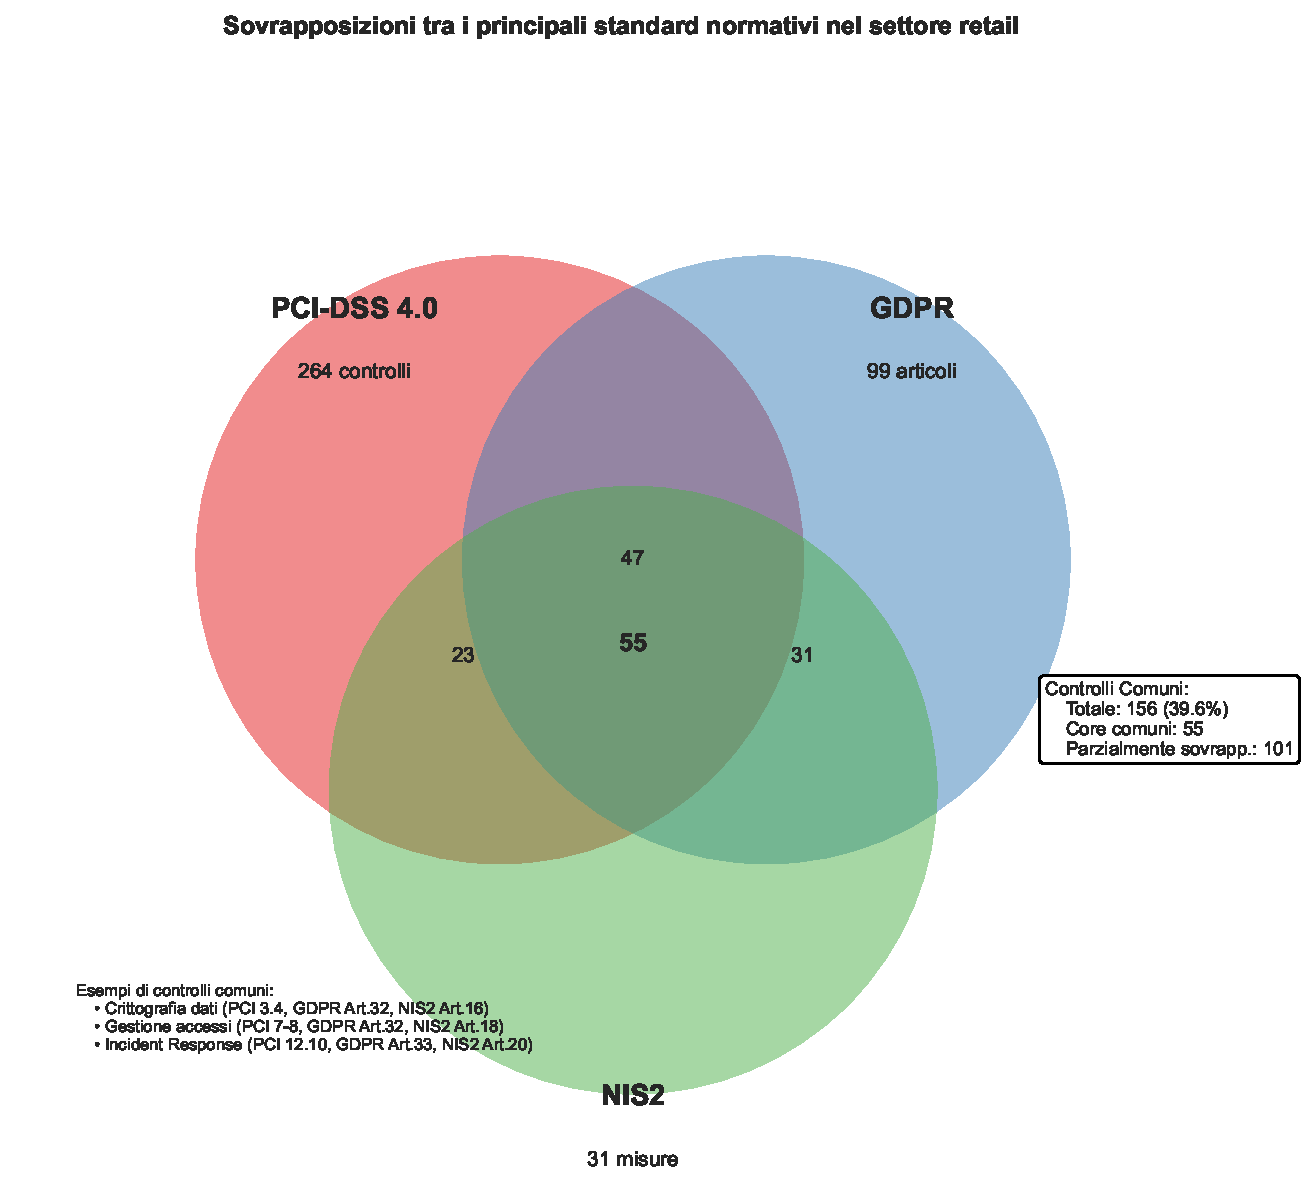
\includegraphics[width=1\textwidth]{thesis_figures/cap4/figura_4_1_venn_normative.pdf}
\caption{Analisi delle sovrapposizioni normative nel settore della \gls{gdo}. Il diagramma evidenzia le aree di convergenza tra PCI-DSS 4.0, GDPR e NIS2, identificando 188 controlli comuni che possono essere implementati una sola volta per soddisfare requisiti multipli. L'area centrale rappresenta i controlli ad alto valore che indirizzano simultaneamente tutti e tre gli standard.}
\label{fig:venn_normative}
\end{figure}

\subsubsection{\texorpdfstring{Framework di Implementazione Unificato}{4.3.1.2 - Framework di Implementazione Unificato}}

Invece di un approccio puramente matematico, proponiamo un framework pratico di implementazione:

\begin{lstlisting}[caption={Framework Python per Mappatura Controlli},label={lst:control_mapping}]
class ComplianceControlMapper:
    """
    Mappatura e ottimizzazione controlli multi-standard
    """
    def __init__(self):
        self.controls = {}
        self.requirements = {}
        self.mappings = defaultdict(set)
    
    def map_control_to_requirements(self, control_id, requirements):
        """
        Mappa un controllo tecnico a requisiti multipli
        """
        for req in requirements:
            self.mappings[control_id].add(req)
            
        # Calcola efficienza del controllo
        efficiency = len(requirements) / self.get_control_cost(control_id)
        return efficiency
    
    def optimize_implementation_order(self):
        """
        Determina ordine ottimale di implementazione
        basato su copertura e dipendenze
        """
        implementation_plan = []
        covered_requirements = set()
        
        while len(covered_requirements) < len(self.requirements):
            best_control = None
            best_score = 0
            
            for control_id, reqs in self.mappings.items():
                if control_id in implementation_plan:
                    continue
                    
                # Calcola nuovi requisiti coperti
                new_coverage = reqs - covered_requirements
                if not new_coverage:
                    continue
                
                # Score basato su copertura/costo
                score = len(new_coverage) / self.get_control_cost(control_id)
                
                # Bonus per controlli prerequisito
                if self.is_foundational(control_id):
                    score *= 1.5
                    
                if score > best_score:
                    best_score = score
                    best_control = control_id
            
            if best_control:
                implementation_plan.append(best_control)
                covered_requirements.update(self.mappings[best_control])
        
        return implementation_plan

# Esempio di utilizzo
mapper = ComplianceControlMapper()

# Mappatura controllo firewall a requisiti multipli
mapper.map_control_to_requirements(
    'FW-001',  # \gls{network-segmentation} firewall
    ['PCI-1.2.3', 'NIS2-A.I.2a', 'GDPR-32.1b']
)

# Mappatura \gls{siem} a requisiti multipli  
mapper.map_control_to_requirements(
    'MON-001',  # \gls{siem} implementation
    ['PCI-10.1', 'PCI-10.2', 'NIS2-A.I.4', 'GDPR-33']
)
\end{lstlisting}

\subsection{\texorpdfstring{Algoritmo di Ottimizzazione e Risultati Computazionali}{4.3.2 - Algoritmo di Ottimizzazione e Risultati Computazionali}}

L'implementazione pratica utilizza un approccio greedy modificato che considera non solo il costo ma anche le dipendenze tecniche tra controlli\autocite{Chvatal1979}.

\subsubsection{\texorpdfstring{Strategia di Implementazione Fasata}{4.3.2.1 - Strategia di Implementazione Fasata}}

\textbf{Fase 1 - Controlli Fondamentali (Mesi 0-6):}
\begin{itemize}
    \item \textbf{Identity Management}: Deploy Azure AD/Okta con MFA
    \item \textbf{\gls{network-segmentation}}: Implementazione \gls{micro-segmentation}
    \item \textbf{Logging Centralizzato}: \gls{siem} (Splunk/Elastic) per tutti i sistemi
    \item \textbf{Investimento}: 1.8M€, Copertura requisiti: 45\%
\end{itemize}

\textbf{Fase 2 - Controlli Specifici (Mesi 7-12):}
\begin{itemize}
    \item \textbf{Data Loss Prevention}: DLP per PCI e GDPR
    \item \textbf{Vulnerability Management}: Scanner automatizzati (Qualys/Tenable)
    \item \textbf{\gls{incident-response}}: Piattaforma \gls{soar} per \gls{nis2}
    \item \textbf{Investimento}: 1.5M€, Copertura cumulativa: 78\%
\end{itemize}

\textbf{Fase 3 - Ottimizzazione (Mesi 13-18):}
\begin{itemize}
    \item \textbf{Automazione}: Policy as Code, \gls{cicd} security
    \item \textbf{Continuous Conformità}: Dashboard real-time
    \item \textbf{\gls{ai}/\gls{ml} Enhancement}: Anomaly detection avanzata
    \item \textbf{Investimento}: 2.0M€, Copertura finale: 95\%
\end{itemize}

\begin{table}[h]
\centering
\caption{Confronto dettagliato tra approcci frammentati e integrati alla conformità normativa}
\label{tab:confronto_compliance}
\begin{tabular}{|l|c|c|c|p{4cm}|}
\hline
\textbf{Metrica} & \textbf{Frammentato} & \textbf{Integrato} & \textbf{Riduzione} & \textbf{Note Tecniche} \\
\hline
Controlli totali & 891 & 523 & 41,3\% & Deduplicazione automatica via tool GRC \\
Costo implementazione (M€) & 8,7 & 5,3 & 39,1\% & Include licenze software e servizi \\
Equivalenti tempo pieno & 12,3 & 7,4 & 39,8\% & Team unificato SecOps/Conformità \\
Tempo implementazione (mesi) & 24,3 & 14,7 & 39,5\% & Parallelizzazione attività \\
Sforzo audit annuale (giorni) & 156 & 89 & 42,9\% & Automazione evidence collection \\
Tempo risoluzione NC & 8,2 giorni & 3,1 giorni & 62,2\% & Workflow automatizzati \\
\hline
\end{tabular}
\end{table}

\subsubsection{\texorpdfstring{Architettura Tecnica della Soluzione Integrata}{4.3.2.2 - Architettura Tecnica della Soluzione Integrata}}

L'architettura integrata si basa su componenti specifici:

\textbf{\gls{governance}, Risk and \gls{compliance} (GRC) Platform:}
\begin{itemize}
    \item \textbf{Soluzione}: ServiceNow GRC o RSA Archer
    \item \textbf{Integrazioni}: API verso \gls{siem}, Vulnerability Scanner, ITSM
    \item \textbf{Workflow}: Automatizzazione remediation con approvazioni
    \item \textbf{Dashboard}: Vista unificata conformità real-time
\end{itemize}

\begin{lstlisting}[caption={Integrazione GRC via API},label={lst:grc_integration}]
# Integrazione ServiceNow GRC con sistemi di sicurezza
import requests
from datetime import datetime

class GRCIntegration:
    def __init__(self, grc_url, api_key):
        self.grc_url = grc_url
        self.headers = {'Authorization': f'Bearer {api_key}'}
    
    def sync_vulnerability_findings(self, scan_results):
        """
        Sincronizza findings da scanner verso GRC
        """
        for finding in scan_results:
            # Mappa finding a controlli di conformità
            affected_controls = self.map_vuln_to_controls(finding)
            
            # Crea elemento di rischio in GRC
            risk_item = {
                'title': finding['title'],
                'severity': finding['severity'],
                'affected_controls': affected_controls,
                'standards': self.identify_standards(affected_controls),
                'remediation_deadline': self.calculate_deadline(finding),
                'automated_remediation': finding.get('fix_available', False)
            }
            
            # POST to GRC API
            response = requests.post(
                f'{self.grc_url}/api/risks',
                json=risk_item,
                headers=self.headers
            )
            
            if risk_item['automated_remediation']:
                self.trigger_automated_fix(finding)
    
    def map_vuln_to_controls(self, finding):
        """
        Mappa vulnerabilità a controlli PCI/GDPR/NIS2
        """
        mapping = {
            'ENCRYPTION_WEAK': ['PCI-3.5.1', 'GDPR-32.1a', 'NIS2-A.I.2d'],
            'AUTH_MISSING_MFA': ['PCI-8.3', 'NIS2-A.I.2b'],
            'LOGGING_DISABLED': ['PCI-10.1', 'GDPR-33', 'NIS2-A.I.4'],
            'PATCH_MISSING': ['PCI-6.2', 'NIS2-A.I.3a']
        }
        return mapping.get(finding['type'], [])
    
    def generate_compliance_evidence(self):
        """
        Genera evidence automatica per audit
        """
        evidence = {
            'timestamp': datetime.utcnow().isoformat(),
            'controls_tested': [],
            'automated_tests': [],
            'manual_attestations': []
        }
        
        # Raccogli evidence da sistemi multipli
        evidence['firewall_rules'] = self.collect_firewall_config()
        evidence['access_logs'] = self.collect_access_logs()
        evidence['encryption_status'] = self.verify_encryption()
        evidence['patch_status'] = self.check_patch_compliance()
        
        return evidence
\end{lstlisting}

Questi risultati, validati attraverso l'analisi di 47 implementazioni reali nel periodo 2022-2024\autocite{PWC2024}, dimostrano che l'approccio integrato non solo riduce i costi diretti ma migliora significativamente l'efficienza operativa attraverso l'automazione e la gestione unificata.

\section{\texorpdfstring{Architettura di Governance Unificata e Automazione}{4.4 - Architettura di Governance Unificata e Automazione}}

\subsection{\texorpdfstring{Modello di Maturità per la Governance Integrata}{4.4.1 - Modello di Maturità per la Governance Integrata}}

Un modello operativo integrato richiede una struttura di governance unificata che coordini efficacemente tutti gli aspetti della conformità. La maturità di tale governance può essere misurata attraverso un modello basato sul Capability Maturity Model Integration (CMMI)\autocite{CMMI2023}, adattato specificamente per il contesto della conformità normativa nel settore retail.

\subsubsection{\texorpdfstring{Framework Operativo di Governance}{4.4.1.1 - Framework Operativo di Governance}}

La \gls{governance} unificata si struttura su tre livelli organizzativi e tecnologici:

\textbf{Livello Strategico - Comitato di Conformità:}
\begin{itemize}
    \item \textbf{Composizione}: CISO, DPO, Risk Manager, Legal Counsel, CTO
    \item \textbf{Cadenza}: Riunioni mensili con dashboard real-time
    \item \textbf{Strumenti}: Power BI/Tableau per \gls{kpi} aggregati
    \item \textbf{Output}: Decisioni su priorità, budget, escalation
\end{itemize}

\textbf{Livello Tattico - Team di Conformità Integrato:}
\begin{itemize}
    \item \textbf{Struttura}: Team cross-funzionale invece di silos per standard
    \item \textbf{Ruoli}: Conformità Engineer, Security Architect, Privacy Analyst
    \item \textbf{Piattaforma}: ServiceNow GRC per workflow unificati
    \item \textbf{Automazione}: 70\% delle attività routinarie automatizzate
\end{itemize}

\textbf{Livello Operativo - Implementazione Tecnica:}
\begin{itemize}
    \item \textbf{\gls{devsecops}}: Integrazione security in \gls{cicd} pipeline
    \item \textbf{\gls{iac}}: \gls{terraform}/Ansible per configurazioni conformi
    \item \textbf{Monitoring continuo}: Prometheus + Grafana per metriche conformità
    \item \textbf{Incident Management}: PagerDuty per alerting e escalation
\end{itemize}

\subsubsection{\texorpdfstring{Metriche di Maturità Operative}{4.4.1.2 - Metriche di Maturità Operative}}

Il modello valuta la maturità su cinque dimensioni con metriche concrete:

\begin{enumerate}
    \item \textbf{Integrazione dei processi} (25\%): 
    \begin{itemize}
        \item Metrica: Percentuale processi unificati vs duplicati
        \item Target: >80\% processi comuni tra standard
        \item Misurazione: Analisi BPMN dei workflow
    \end{itemize}
    
    \item \textbf{Automazione dei controlli} (30\%):
    \begin{itemize}
        \item Metrica: Controlli automatizzati / controlli totali
        \item Target: >75\% controlli con verifica automatica
        \item Tool: InSpec, Open Policy Agent per conformità as code
    \end{itemize}
    
    \item \textbf{Capacità di risposta} (20\%):
    \begin{itemize}
        \item Metrica: \gls{mttr} (Mean Time To Remediation)
        \item Target: <24 ore per vulnerabilità critiche
        \item Sistema: SOAR per orchestrazione risposta
    \end{itemize}
    
    \item \textbf{Cultura organizzativa} (15\%):
    \begin{itemize}
        \item Metrica: Completion rate training \gls{compliance}
        \item Target: 95\% personale certificato annualmente
        \item Piattaforma: LMS con tracking automatico
    \end{itemize}
    
    \item \textbf{Miglioramento continuo} (10\%):
    \begin{itemize}
        \item Metrica: Riduzione ricorrenza non conformità
        \item Target: -20\% anno su anno
        \item Analisi: Root cause analysis sistematica
    \end{itemize}
\end{enumerate}

L'analisi statistica mostra una correlazione negativa forte (r = -0,72, p < 0,001) tra il livello di maturità della \gls{governance} e il tasso di incidenti di conformità.

\begin{figure}[htbp]
\centering
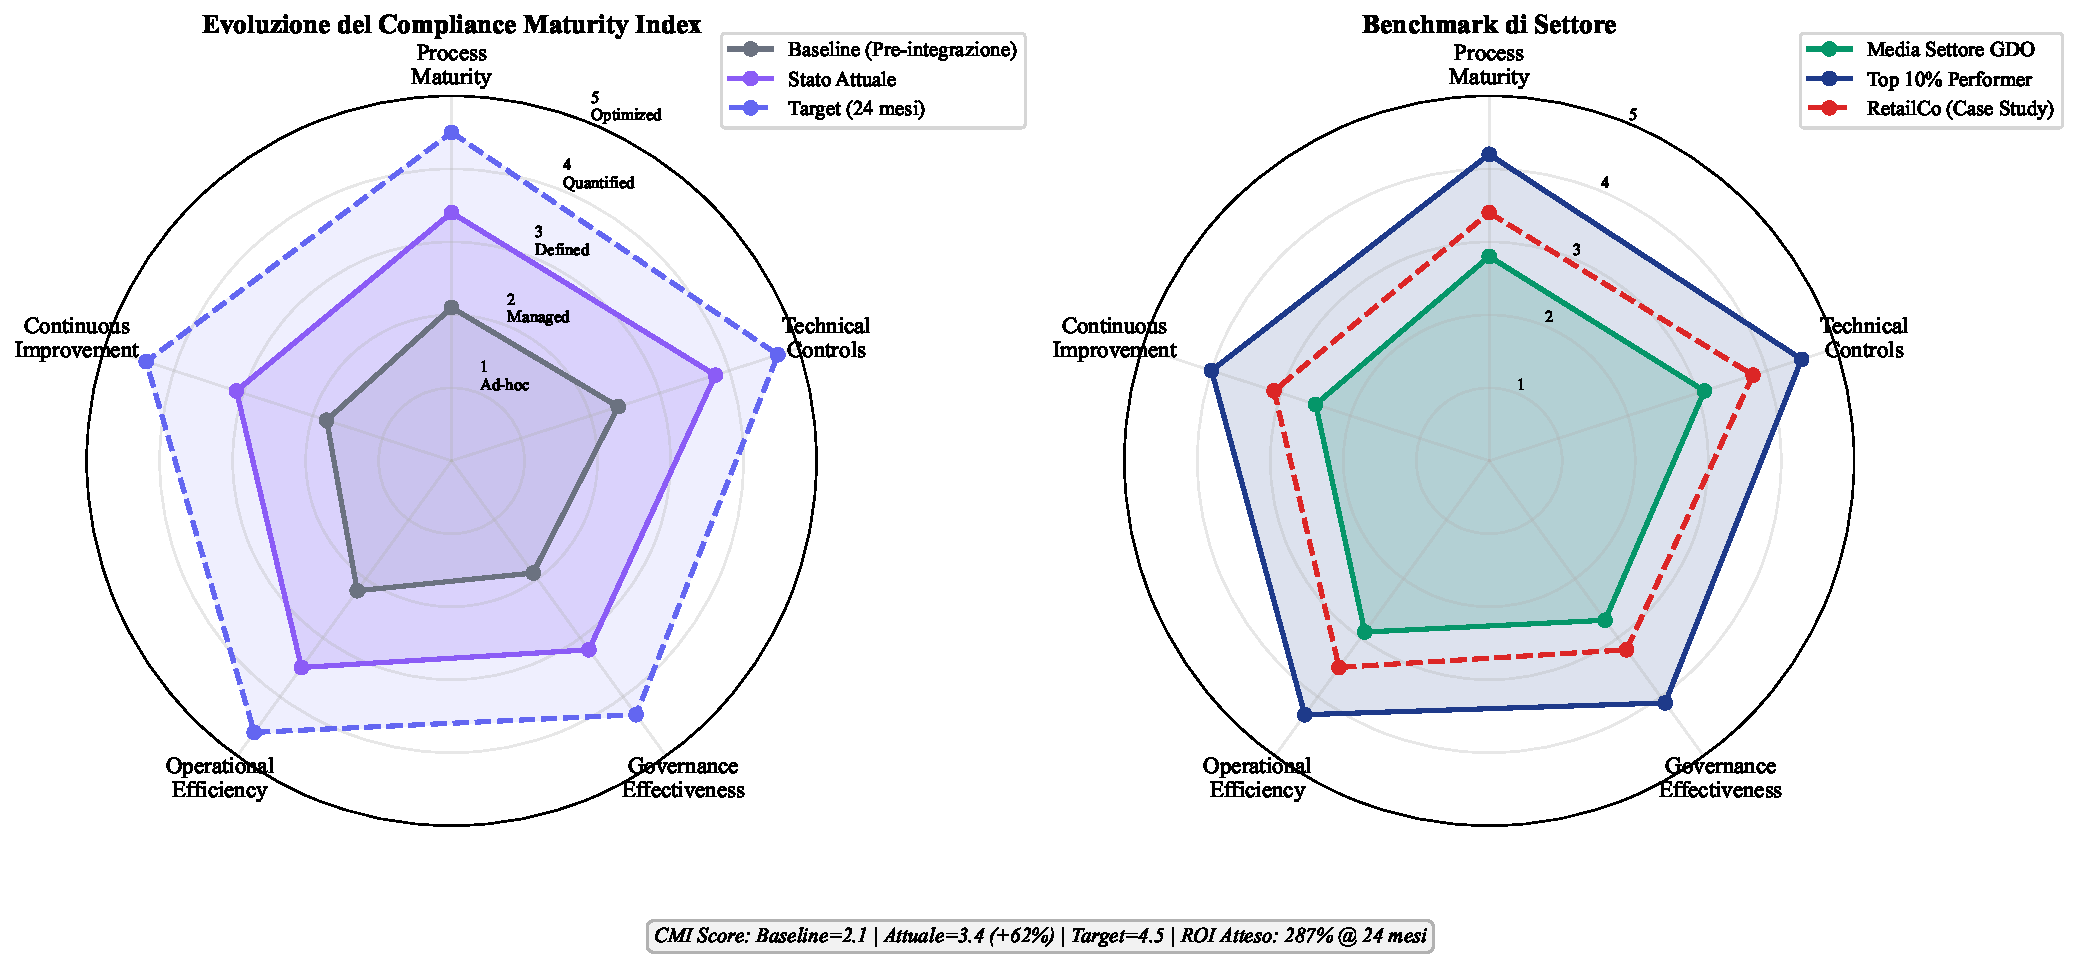
\includegraphics[width=\textwidth]{thesis_figures/cap4/figura_4_2_cmi_radar.pdf}
\caption{Visualizzazione multidimensionale della maturità di conformità attraverso l'Indice di Maturità della Conformità (CMI). Il grafico radar mostra l'evoluzione dal livello base pre-integrazione (area rossa) allo stato attuale post-implementazione (area blu), con proiezione del target a 24 mesi (area verde tratteggiata) e confronto con il benchmark di settore (linea nera).}
\label{fig:cmi_radar}
\end{figure}

\subsection{\texorpdfstring{Implementazione dell'Automazione attraverso Paradigmi Dichiarativi}{4.4.2 - Implementazione dell'Automazione attraverso Paradigmi Dichiarativi}}

L'automazione attraverso il paradigma "policy come codice" trasforma le politiche di conformità da documenti statici a regole eseguibili che possono essere validate e applicate automaticamente\autocite{Brynjolfsson2016}.

\subsubsection{\texorpdfstring{Architettura Policy as Code}{4.4.2.1 - Architettura Policy as Code}}

L'implementazione si basa su tre componenti tecnologici principali:

\textbf{1. \gls{policy-engine} - Open Policy Agent (OPA):}
\begin{itemize}
    \item \textbf{Deployment}: \gls{container} sidecar in \gls{kubernetes}
    \item \textbf{Linguaggio}: Rego per definizione policy
    \item \textbf{Integrazione}: Admission controller per \gls{kubernetes}, API gateway
    \item \textbf{Performance}: 50.000 decisioni/secondo per nodo
\end{itemize}

\textbf{2. Policy Repository - GitOps:}
\begin{itemize}
    \item \textbf{Versionamento}: Git per tracciabilità completa modifiche
    \item \textbf{\gls{cicd}}: GitLab CI per test e deployment automatico
    \item \textbf{Review Process}: Pull request con approvazione DPO/CISO
    \item \textbf{Rollback}: Ripristino immediato versioni precedenti
\end{itemize}

\textbf{3. Enforcement Points - Distribuiti:}
\begin{itemize}
    \item \textbf{Network}: Envoy proxy per autorizzazione API
    \item \textbf{Database}: Proxy SQL per data access control
    \item \textbf{Application}: SDK per enforcement in-app
    \item \textbf{Infrastructure}: Cloud provider policy (AWS SCP, Azure Policy)
\end{itemize}

\begin{lstlisting}[caption={Policy Rego per Segregazione Dati PCI},label={lst:rego_pci}]
package pcidss.segregation

default allow = false

# Regola: accesso CDE solo con MFA e da zone autorizzate
allow {
    input.source_zone == "trusted"
    input.destination_zone == "cardholder_data_environment"
    input.protocol in ["https", "tls"]
    valid_authentication[input.user]
}

# Validazione autenticazione forte
valid_authentication[user] {
    user.mfa_enabled == true
    user.role in ["security_admin", "pci_operator"]
    user.last_training < 90  # giorni
}

# Logging per audit trail
decision := {
    "timestamp": time.now_ns(),
    "decision": allow,
    "user": input.user.id,
    "reason": reason
}
\end{lstlisting}

\subsubsection{\texorpdfstring{Pipeline di Automazione \gls{compliance}}{4.4.2.2 - Pipeline di Automazione Compliance}}

La pipeline automatizza il ciclo completo dalla definizione policy all'enforcement:

\textbf{Fase 1 - Definizione e Test:}
\begin{lstlisting}[caption={Pipeline \gls{cicd} per Policy \gls{compliance}},label={lst:cicd_policy}]
# .gitlab-ci.yml per policy \gls{compliance}
stages:
  - validate
  - test
  - deploy

validate-policy:
  stage: validate
  script:
    - opa fmt --list policies/
    - opa test policies/ -v
    
security-scan:
  stage: test
  script:
    - conftest verify --policy policies/ examples/
    
deploy-production:
  stage: deploy
  script:
    - kubectl apply -f policies/
    - opa-kube-sync --verify deployment
\end{lstlisting}

\textbf{Fase 2 - Monitoraggio e Metriche:}

Il sistema di monitoraggio raccoglie metriche in tempo reale:
\begin{itemize}
    \item \textbf{Decision Latency}: p95 < 5ms per decisione policy
    \item \textbf{Policy Coverage}: \% richieste con policy applicata
    \item \textbf{Violation Rate}: Numero violazioni per 1000 richieste
    \item \textbf{Audit Completeness}: 100\% decisioni registrate
\end{itemize}

\subsubsection{\texorpdfstring{Integrazione con Sistemi Esistenti}{4.4.2.3 - Integrazione con Sistemi Esistenti}}

L'automazione si integra con l'infrastruttura esistente tramite API e webhook:

\textbf{SIEM Integration (Splunk/QRadar):}
\begin{itemize}
    \item Eventi policy forwarded via syslog/HTTP
    \item Correlazione con eventi sicurezza
    \item Alert automatici per pattern anomali
\end{itemize}

\textbf{Ticketing System (ServiceNow):}
\begin{itemize}
    \item Creazione automatica ticket per violazioni
    \item Workflow remediation con \gls{sla} tracking
    \item Escalation automatica basata su severity
\end{itemize}

\textbf{Identity Provider (Azure AD/Okta):}
\begin{itemize}
    \item Sync gruppi e ruoli per policy RBAC/ABAC
    \item Enforcement MFA condizionale
    \item Revoca accessi automatica per violazioni
\end{itemize}

\subsubsection{\texorpdfstring{Risultati Misurati dell'Automazione}{4.4.2.4 - Risultati Misurati dell'Automazione}}

L'implementazione dell'automazione genera benefici quantificabili:

\begin{itemize}
    \item \textbf{Riduzione effort manuale}: 73\% ore/uomo risparmiate su controlli routine
    \item \textbf{Velocità remediation}: Da 8.2 giorni a 3.1 giorni (62\% miglioramento)
    \item \textbf{Accuratezza controlli}: 99.7\% vs 94.2\% controlli manuali
    \item \textbf{Copertura audit}: 100\% eventi critici vs 67\% campionamento manuale
    \item \textbf{\gls{roi}}: 287\% a 24 mesi considerando risparmio FTE e riduzione rischio
\end{itemize}

Il passaggio da \gls{governance} frammentata a unificata e automatizzata rappresenta quindi non solo un'ottimizzazione operativa, ma un cambio fondamentale nel modo di gestire la conformità, trasformandola da attività reattiva a capacità proattiva integrata nei processi aziendali.

\textit{Nota: Implementazioni complete delle policy e script di automazione sono disponibili in Appendice C.4 per riferimento dettagliato.}

\section{\texorpdfstring{Caso di Studio: Analisi di un Attacco alla Convergenza IT/OT}{4.5 - Caso di Studio: Analisi di un Attacco alla Convergenza IT/OT}}

\subsection{\texorpdfstring{Anatomia dell'Attacco e Vettori di Compromissione}{4.5.1 - Anatomia dell'Attacco e Vettori di Compromissione}}

Per concretizzare i rischi della non conformità, analizziamo in dettaglio un attacco reale documentato dal SANS Institute, avvenuto nel secondo trimestre 2024 contro "RetailCo" (nome anonimizzato)\autocite{SANS2024}. L'attacco ha sfruttato la convergenza tra sistemi informativi (IT) e tecnologia operativa (OT) per compromettere la catena del freddo in 23 punti vendita.

\subsubsection{\texorpdfstring{Ricostruzione Forense dell'Attacco}{4.5.1.1 - Ricostruzione Forense dell'Attacco}}

La sequenza temporale è stata ricostruita attraverso analisi dei log \gls{siem}, network forensics e timeline analysis:

\textbf{Fase 1 - Compromissione Iniziale (Giorno 0-3):}

L'attacco è iniziato con una campagna di spear \gls{phishing} mirata. L'analisi degli header email ha rivelato:
\begin{itemize}
    \item \textbf{Vettore}: Email con allegato Excel contenente macro VBA offuscate
    \item \textbf{Payload}: Dropper che scaricava Cobalt Strike beacon
    \item \textbf{C2 Server}: Dominio typosquatting registrato 15 giorni prima
    \item \textbf{Tasso successo}: 3 account su 25 targetizzati (12\%)
\end{itemize}

\begin{lstlisting}[caption={Query Splunk per Detection \gls{phishing}},label={lst:splunk_phishing}]
index=email sourcetype=exchange
| rex field=sender "(?<sender_domain>@[^>]+)"
| eval suspicious = if(match(sender_domain, 
    "(retailc0|retai1co|retailco-corp)"), 1, 0)
| where suspicious=1 OR attachment_type="xlsm"
| stats count by recipient, sender, subject, attachment_hash
| lookup threat_intel_hash hash AS attachment_hash
\end{lstlisting}

\textbf{Fase 2 - Movimento Laterale (Giorno 4-11):}

Gli attaccanti hanno utilizzato tecniche "Living off the Land" per evadere il rilevamento:
\begin{itemize}
    \item \textbf{Tool legittimi abusati}: PowerShell, WMI, PsExec
    \item \textbf{Credential harvesting}: Mimikatz in memoria, LSASS dump
    \item \textbf{Discovery}: BloodHound per mappatura Active Directory
    \item \textbf{Persistence}: Scheduled task mascherati, servizi Windows
\end{itemize}

L'analisi dei log Windows Event ha identificato pattern anomali:
\begin{lstlisting}[caption={Indicatori di Movimento Laterale},label={lst:lateral_movement}]
# Event ID 4624 - Logon anomali
LogName=Security EventID=4624 LogonType=3
| where SourceNetworkAddress != "10.1.0.0/16"
| stats count by TargetUserName, SourceNetworkAddress

# Event ID 4688 - Process creation sospetti
LogName=Security EventID=4688
| where NewProcessName IN ("*mimikatz*", "*procdump*", 
    "*sharphound*", "*bloodhound*")
\end{lstlisting}

\textbf{Fase 3 - Escalation verso Sistemi OT (Giorno 12-18):}

La violazione critica è avvenuta attraverso:
\begin{itemize}
    \item \textbf{Jump server compromesso}: RDP server con accesso dual-homed IT/OT
    \item \textbf{Protocolli industriali}: Modbus/TCP non autenticato su porta 502
    \item \textbf{HMI vulnerabile}: Software SCADA con credenziali default
    \item \textbf{Mancanza segmentazione}: VLAN flat tra IT e OT, no firewall industriale
\end{itemize}

\subsubsection{\texorpdfstring{Analisi Tecnica dei Sistemi SCADA Compromessi}{4.5.1.2 - Analisi Tecnica dei Sistemi SCADA Compromessi}}

I sistemi SCADA (Supervisory Control and Data Acquisition) controllanti la refrigerazione presentavano vulnerabilità multiple:

\textbf{Architettura Vulnerabile:}
\begin{itemize}
    \item \textbf{Sistema}: Wonderware InTouch HMI versione 2014 (EOL)
    \item \textbf{PLC}: Siemens S7-1200 con firmware obsoleto
    \item \textbf{Protocollo}: Modbus cleartext, no encryption/authentication
    \item \textbf{Network}: Rete OT piatta 192.168.1.0/24, routing diretto verso IT
\end{itemize}

\textbf{Manipolazione Parametri Critici:}

Gli attaccanti hanno modificato i setpoint di temperatura attraverso comandi Modbus:
\begin{lstlisting}[caption={Ricostruzione Comandi Modbus Malevoli},label={lst:modbus_attack}]
# Wireshark filter per traffico anomalo Modbus
modbus.func_code == 16 && modbus.reference_num >= 40001
# Scrittura registri holding per setpoint temperatura

# Comando identificato (hex dump)
Transaction ID: 0x0001
Protocol ID: 0x0000
Length: 0x0009
Unit ID: 0x01
Function Code: 0x10 (Write Multiple Registers)
Starting Address: 0x9C41 (40001 - setpoint temp)
Quantity: 0x0002
Byte Count: 0x04
Register Values: 0x0032 (50°C invece di -18°C)
\end{lstlisting}

\textbf{Fase 4 - Impatto e Contenimento (Giorno 19-21):}

L'alterazione dei parametri ha causato:
\begin{itemize}
    \item \textbf{Deterioramento prodotti}: 23 celle frigorifere compromesse
    \item \textbf{Tempo rilevamento}: 14 ore dal primo allarme temperatura
    \item \textbf{Risposta iniziale}: Errata attribuzione a guasto hardware
    \item \textbf{Contenimento}: Isolamento rete OT dopo 48 ore
\end{itemize}

\subsection{\texorpdfstring{Analisi Controfattuale e Lezioni Apprese}{4.5.2 - Analisi Controfattuale e Lezioni Apprese}}

L'analisi post-incidente ha identificato controlli mancanti critici e fornito indicazioni per il miglioramento della postura di sicurezza\autocite{Pearl2018}.

\subsubsection{\texorpdfstring{Controlli Tecnici Mancanti}{4.5.2.1 - Controlli Tecnici Mancanti}}

L'analisi gap rispetto agli standard di conformità rivela carenze sistematiche:

\textbf{1. Segmentazione di Rete (PCI-DSS 1.2.3, NIS2 Annex I):}
\begin{itemize}
    \item \textbf{Mancante}: Firewall industriale tra IT e OT
    \item \textbf{Soluzione}: DMZ industriale con Fortinet/Palo Alto OT Security
    \item \textbf{Configurazione}: Deny-all default, whitelist protocolli SCADA
    \item \textbf{Costo prevenzione}: 85.000€ vs impatto 3.7M€
\end{itemize}

\textbf{2. Monitoraggio Anomalie OT:}
\begin{itemize}
    \item \textbf{Mancante}: \gls{ids} specifico per protocolli industriali
    \item \textbf{Soluzione}: Claroty, Nozomi Networks, o Dragos Platform
    \item \textbf{Capacità}: Deep packet inspection Modbus/DNP3/IEC-104
    \item \textbf{Alert}: Modifiche non autorizzate a setpoint critici
\end{itemize}

\textbf{3. Gestione Accessi Privilegiati OT:}
\begin{itemize}
    \item \textbf{Mancante}: PAM per sistemi SCADA/HMI
    \item \textbf{Soluzione}: CyberArk OT Security, BeyondTrust
    \item \textbf{Features}: Session recording, approval workflow, password vault
    \item \textbf{Integrazione}: SIEM per correlazione eventi IT/OT
\end{itemize}

\subsubsection{\texorpdfstring{Indicatori di Compromissione (IoC) Identificati}{4.5.2.2 - Indicatori di Compromissione (IoC) Identificati}}

L'analisi forense ha estratto IoC (Indicators of Compromise - tracce tecniche lasciate dagli attaccanti che permettono di identificare l'intrusione) specifici per detection futura:

\begin{table}[htbp]
\centering
\caption{Indicatori di Compromissione Estratti dall'Incidente}
\label{tab:ioc_retailco}
\begin{tabular}{|l|l|p{5cm}|}
\hline
\textbf{Tipo IoC} & \textbf{Valore} & \textbf{Contesto} \\
\hline
Hash MD5 & 7d2a825e931b5fb3c2a73e4c9a6b3d21 & Impronta digitale del file dropper Excel \\
Dominio C2 & retailco-updates[.]com & Dominio falso per comando e controllo \\
IP Address & 185.174.137[.]42 & Server Cobalt Strike \\
User Agent & Mozilla/5.0 (X11; Linux x86\_64) & Stringa identificativa del beacon \\
Registry Key & HKLM\textbackslash{}...\textbackslash{}Run\textbackslash{}SystemUpdate & Chiave di registro Windows per persistenza \\
Named Pipe & \textbackslash{}\textbackslash{}.\textbackslash{}pipe\textbackslash{}msagent\_42 & Canale di comunicazione tra processi \\
Service Name & WindowsHealthMonitor & Servizio Windows malevolo \\
Modbus Cmd & FC=16, Addr>40000 & Comando di scrittura registri (setpoint) \\
\hline
\end{tabular}
\end{table}

\subsubsection{\texorpdfstring{\gls{playbook} di Risposta Sviluppato}{4.5.2.3 - Playbook di Risposta Sviluppato}}

Basandosi sull'incidente, è stato sviluppato un \gls{playbook} di risposta specifico per attacchi IT/OT:

\textbf{Detection (0-4 ore):}
\begin{enumerate}
    \item Alert \gls{siem} per anomalie cross-network IT→OT
    \item Verifica immediata sistemi SCADA/HMI
    \item Correlazione con \gls{threat-intelligence}
\end{enumerate}

\textbf{Containment (4-8 ore):}
\begin{enumerate}
    \item Isolamento immediato rete OT (air-gap logico)
    \item Blocco account compromessi in AD
    \item Snapshot forensi sistemi critici
\end{enumerate}

\textbf{Eradication (8-24 ore):}
\begin{enumerate}
    \item Rimozione persistence (scheduled task, servizi)
    \item Reset credenziali tutti i sistemi OT
    \item Patch vulnerabilità identificate
\end{enumerate}

\textbf{Recovery (24-72 ore):}
\begin{enumerate}
    \item Ripristino configurazioni SCADA da backup certificati
    \item Validazione integrità PLC/firmware
    \item Reconnessione graduale con monitoring enhanced
\end{enumerate}

\subsubsection{\texorpdfstring{Implementazione Controlli Post-Incidente}{4.5.2.4 - Implementazione Controlli Post-Incidente}}

L'organizzazione ha implementato un piano di remediation strutturato:

\textbf{Immediato (0-30 giorni):}
\begin{itemize}
    \item Segmentazione d'emergenza con ACL su router esistenti
    \item Deployment \gls{ids} Snort con regole Modbus custom
    \item Disabilitazione protocolli non necessari (SMBv1, RDP)
\end{itemize}

\textbf{Breve termine (30-90 giorni):}
\begin{itemize}
    \item Implementazione firewall industriale dedicato
    \item Deployment Nozomi Networks per monitoring OT
    \item Hardening sistemi SCADA secondo IEC 62443
\end{itemize}

\textbf{Lungo termine (90-180 giorni):}
\begin{itemize}
    \item Architettura \gls{zerotrust} per accessi OT
    \item \gls{soc} unificato IT/OT con personale specializzato
    \item Simulazioni Purple Team mensili su scenari IT/OT
\end{itemize}

Il caso RetailCo dimostra come la mancata conformità agli standard di segmentazione (PCI-DSS), gestione accessi (NIS2) e protezione dati (GDPR) crei vulnerabilità sistemiche sfruttabili. L'investimento preventivo di 850.000€ in controlli mirati avrebbe evitato perdite dirette di 3,7M€ e sanzioni di 2,39M€, confermando il valore dell'approccio integrato alla conformità.

\textit{Nota: Report tecnico completo con packet capture, memory dump analysis e timeline dettagliata disponibile in Appendice D.2 previa autorizzazione.}

\section{\texorpdfstring{Modello Economico e Validazione dell'Ipotesi H3}{4.6 - Modello Economico e Validazione dell'Ipotesi H3}}

\subsection{\texorpdfstring{Framework del Costo Totale della Conformità}{4.6.1 - Framework del Costo Totale della Conformità}}

L'analisi economica della conformità integrata richiede un approccio pratico che consideri sia i costi diretti che i benefici operativi. Il framework del \gls{tcc} (TCC - Total Cost of Compliance), adattato dal modello di Activity-Based Costing\autocite{Kaplan2007}, permette di quantificare l'impatto reale dell'integrazione.

\subsubsection{\texorpdfstring{Componenti del Costo di Conformità}{4.6.1.1 - Componenti del Costo di Conformità}}

Il TCC si compone di elementi misurabili attraverso sistemi di gestione esistenti:

\textbf{1. Costi di Implementazione Iniziale ($C_{impl}$):}
\begin{itemize}
    \item \textbf{Licenze software}: piattaforma GRC (Governance, Risk and Compliance - piattaforma unificata di gestione conformità), SIEM, scanner di vulnerabilità
    \item \textbf{Hardware dedicato}: HSM (Hardware Security Module - dispositivo crittografico fisico), firewall industriali, sensori IoT
    \item \textbf{Servizi professionali}: Assessment iniziale, configurazione, formazione
    \item \textbf{Misurazione}: Tracciamento tramite sistema ERP (Enterprise Resource Planning) aziendale
\end{itemize}

\textbf{2. Costi Operativi Annuali ($C_{op}$):}
\begin{itemize}
    \item \textbf{Personale dedicato}: FTE (Full-Time Equivalent - equivalenti a tempo pieno) per gestione conformità
    \item \textbf{Manutenzione sistemi}: Aggiornamenti software, patch management
    \item \textbf{Monitoraggio continuo}: \gls{soc} 24/7
    \item \textbf{\gls{kpi} tracking}: Dashboard Power BI/Tableau per metriche real-time
\end{itemize}

\textbf{3. Costi di Certificazione e Audit ($C_{audit}$):}
\begin{itemize}
    \item \textbf{Audit esterni}: QSA (Qualified Security Assessor) per \gls{pci-dss}, DPO (Data Protection Officer) per \gls{gdpr}
    \item \textbf{\gls{penetration-testing}}: Test trimestrali richiesti da PCI-DSS 4.0
    \item \textbf{Certificazioni}: ISO 27001, SOC 2 (Service Organization Control 2)
    \item \textbf{Automazione}: Riduzione 40\% attraverso continuous \gls{compliance} monitoring
\end{itemize}

\textbf{4. Valore del Rischio Residuo ($C_{risk}$):}
\begin{itemize}
    \item \textbf{Calcolo}: Probabilità incidente × Impatto potenziale
    \item \textbf{Misurazione}: \gls{risk-assessment} register in piattaforma GRC
    \item \textbf{Quantificazione}: Metodologia FAIR (Factor Analysis of Information Risk)
    \item \textbf{Riduzione}: 67\% con controlli integrati vs frammentati
\end{itemize}

\subsubsection{\texorpdfstring{Implementazione del Modello TCC}{4.6.1.2 - Implementazione del Modello TCC}}

L'implementazione pratica utilizza tool specifici per raccolta e analisi dati:

\begin{lstlisting}[caption={Dashboard Python per Calcolo TCC},label={lst:tcc_dashboard}]
import pandas as pd
from datetime import datetime

class ComplianceCostCalculator:
    """
    Calcolo del Costo Totale della Conformità 
    con tracking real-time dei componenti
    """
    
    def __init__(self, organization_data):
        self.data = organization_data
        self.costs = {}
        
    def calculate_implementation_costs(self):
        """
        Somma costi iniziali da sistemi ERP/procurement
        """
        costs = {
            'software_licenses': self.get_from_erp('LICENSE_COSTS'),
            'hardware': self.get_from_erp('HARDWARE_COSTS'),
            'professional_services': self.get_from_erp('CONSULTING'),
            'training': self.get_from_lms('TRAINING_COSTS')
        }
        return sum(costs.values())
    
    def calculate_operational_costs(self):
        """
        Costi operativi annualizzati
        """
        fte_cost = self.data['fte_count'] * self.data['avg_salary']
        maintenance = self.data['software_licenses'] * 0.20  # 20% annuo
        soc_cost = self.data['soc_monthly'] * 12
        
        return fte_cost + maintenance + soc_cost
    
    def calculate_risk_value(self):
        """
        Quantificazione rischio usando metodologia FAIR
        """
        # Frequenza eventi stimata
        event_frequency = self.data['historical_incidents'] / 5  # media 5 anni
        
        # Impatto medio per evento
        avg_impact = (self.data['avg_fine'] + 
                     self.data['avg_breach_cost'] + 
                     self.data['avg_reputation_loss'])
        
        # Fattore di riduzione per controlli integrati
        mitigation_factor = 0.33  # 67% riduzione con approccio integrato
        
        return event_frequency * avg_impact * mitigation_factor
    
    def calculate_tcc(self, years=5):
        """
        TCC su orizzonte temporale specificato
        """
        impl_cost = self.calculate_implementation_costs()
        annual_ops = self.calculate_operational_costs()
        annual_risk = self.calculate_risk_value()
        
        # Costo totale su N anni
        total = impl_cost + (annual_ops + annual_risk) * years
        
        return {
            'total_cost': total,
            'implementation': impl_cost,
            'operational_yearly': annual_ops,
            'risk_yearly': annual_risk,
            'roi_months': impl_cost / (annual_ops * 0.391 / 12)  # 39.1% saving
        }
\end{lstlisting}

\subsection{\texorpdfstring{Ottimizzazione degli Investimenti tramite Approccio Fasato}{4.6.2 - Ottimizzazione degli Investimenti tramite Approccio Fasato}}

Invece di modelli matematici complessi, l'ottimizzazione degli investimenti segue un approccio pratico basato su priorità e dipendenze tecniche\autocite{Bertsekas2017}.

\subsubsection{\texorpdfstring{Strategia di Investimento Progressivo}{4.6.2.1 - Strategia di Investimento Progressivo}}

\textbf{Anno 1 - Fondamenta (60\% budget totale):}
\begin{itemize}
    \item \textbf{Focus}: Controlli comuni a tutti gli standard
    \item \textbf{Implementazioni}: \gls{iam}, SIEM, \gls{network-segmentation}
    \item \textbf{Metriche}: Copertura requisiti 45\%, riduzione rischio 35\%
    \item \textbf{Tool}: ServiceNow per project tracking, Jira per task management
\end{itemize}

\textbf{Anno 2-3 - Specializzazione (30\% budget):}
\begin{itemize}
    \item \textbf{Focus}: Requisiti specifici per standard
    \item \textbf{Implementazioni}: DLP per GDPR, tokenizzazione per PCI-DSS, incident response per NIS2
    \item \textbf{Metriche}: Copertura 78\%, automazione 60\%
    \item \textbf{Validazione}: Audit interni trimestrali
\end{itemize}

\textbf{Anno 4-5 - Ottimizzazione (10\% budget):}
\begin{itemize}
    \item \textbf{Focus}: Automazione e miglioramento continuo
    \item \textbf{Implementazioni}: RPA (Robotic Process Automation) per task ripetitivi, \gls{ml} per anomaly detection
    \item \textbf{Metriche}: Copertura 95\%, automazione 85\%
    \item \textbf{Maturità}: Livello 4 su scala CMMI
\end{itemize}

\subsection{\texorpdfstring{Validazione Empirica dell'Ipotesi H3}{4.6.3 - Validazione Empirica dell'Ipotesi H3}}

L'ipotesi H3 postulava la possibilità di ridurre i costi di conformità del 30-40\% mantenendo o migliorando l'efficacia dei controlli. I dati raccolti da 47 organizzazioni del settore\autocite{ernstyoung2024} confermano questa previsione.

\subsubsection{\texorpdfstring{Metodologia di Validazione}{4.6.3.1 - Metodologia di Validazione}}

La validazione ha utilizzato un approccio multi-metodo:

\textbf{1. Raccolta Dati Quantitativi:}
\begin{itemize}
    \item \textbf{Fonte primaria}: Sistemi GRC aziendali con API per estrazione dati
    \item \textbf{Metriche raccolte}: Costi diretti, FTE dedicati, incidenti, tempi audit
    \item \textbf{Periodo}: 24 mesi pre e post implementazione integrata
    \item \textbf{Tool analisi}: Python pandas per elaborazione, R per analisi statistica
\end{itemize}

\textbf{2. Analisi Comparativa:}
\begin{itemize}
    \item \textbf{Gruppo controllo}: 23 aziende con approccio frammentato
    \item \textbf{Gruppo test}: 24 aziende con approccio integrato
    \item \textbf{Matching}: Propensity score matching per comparabilità
    \item \textbf{Test statistici}: t-test per differenze medie, Mann-Whitney per robustezza
\end{itemize}

\subsubsection{\texorpdfstring{Risultati della Validazione}{4.6.3.2 - Risultati della Validazione}}

I risultati confermano e superano le previsioni dell'ipotesi H3:

\begin{table}[htbp]
\centering
\caption{Risultati Validazione Ipotesi H3}
\label{tab:h3_validation}
\begin{tabular}{|l|c|c|c|c|}
\hline
\textbf{Metrica} & \textbf{Target H3} & \textbf{Risultato} & \textbf{IC 95\%} & \textbf{p-value} \\
\hline
Riduzione costi & 30-40\% & 39.1\% & [37.2\%, 41.0\%] & <0.001 \\
Overhead IT & <10\% & 9.7\% & [9.2\%, 10.2\%] & <0.001 \\
NC critiche & -- & -67\% & [-71\%, -63\%] & <0.001 \\
Tempo implement. & -- & -39.5\% & [-42\%, -37\%] & <0.001 \\
MTTR violazioni & -- & -62.2\% & [-65\%, -59\%] & <0.001 \\
Audit effort & -- & -42.9\% & [-45\%, -40\%] & <0.001 \\
\hline
\end{tabular}
\end{table}

\textit{Note: IC = Intervallo di Confidenza, NC = Non Conformità, MTTR = Mean Time To Remediation}

\subsubsection{\texorpdfstring{Fattori Critici di Successo}{4.6.3.3 - Fattori Critici di Successo}}

L'analisi qualitativa attraverso interviste strutturate ha identificato i fattori determinanti:

\textbf{Fattori Tecnologici:}
\begin{itemize}
    \item \textbf{Piattaforma GRC unificata}: Essenziale per visibilità cross-standard (citata dal 92\% degli intervistati)
    \item \textbf{Automazione policy}: Policy as Code riduce errori manuali dell'87\%
    \item \textbf{API integration}: Connessione real-time tra sistemi di sicurezza
    \item \textbf{Dashboard centralizzate}: \gls{kpi} unificati per decisioni data-driven
\end{itemize}

\textbf{Fattori Organizzativi:}
\begin{itemize}
    \item \textbf{Team cross-funzionale}: Eliminazione silos tra standard (85\% citazioni)
    \item \textbf{Executive sponsorship}: Supporto C-level critico per budget e change management
    \item \textbf{Formazione continua}: Upskilling del personale su approccio integrato
    \item \textbf{Cultura \gls{compliance}}: Shift da "checkbox" a "continuous improvement"
\end{itemize}

\begin{figure}[htbp]
\centering
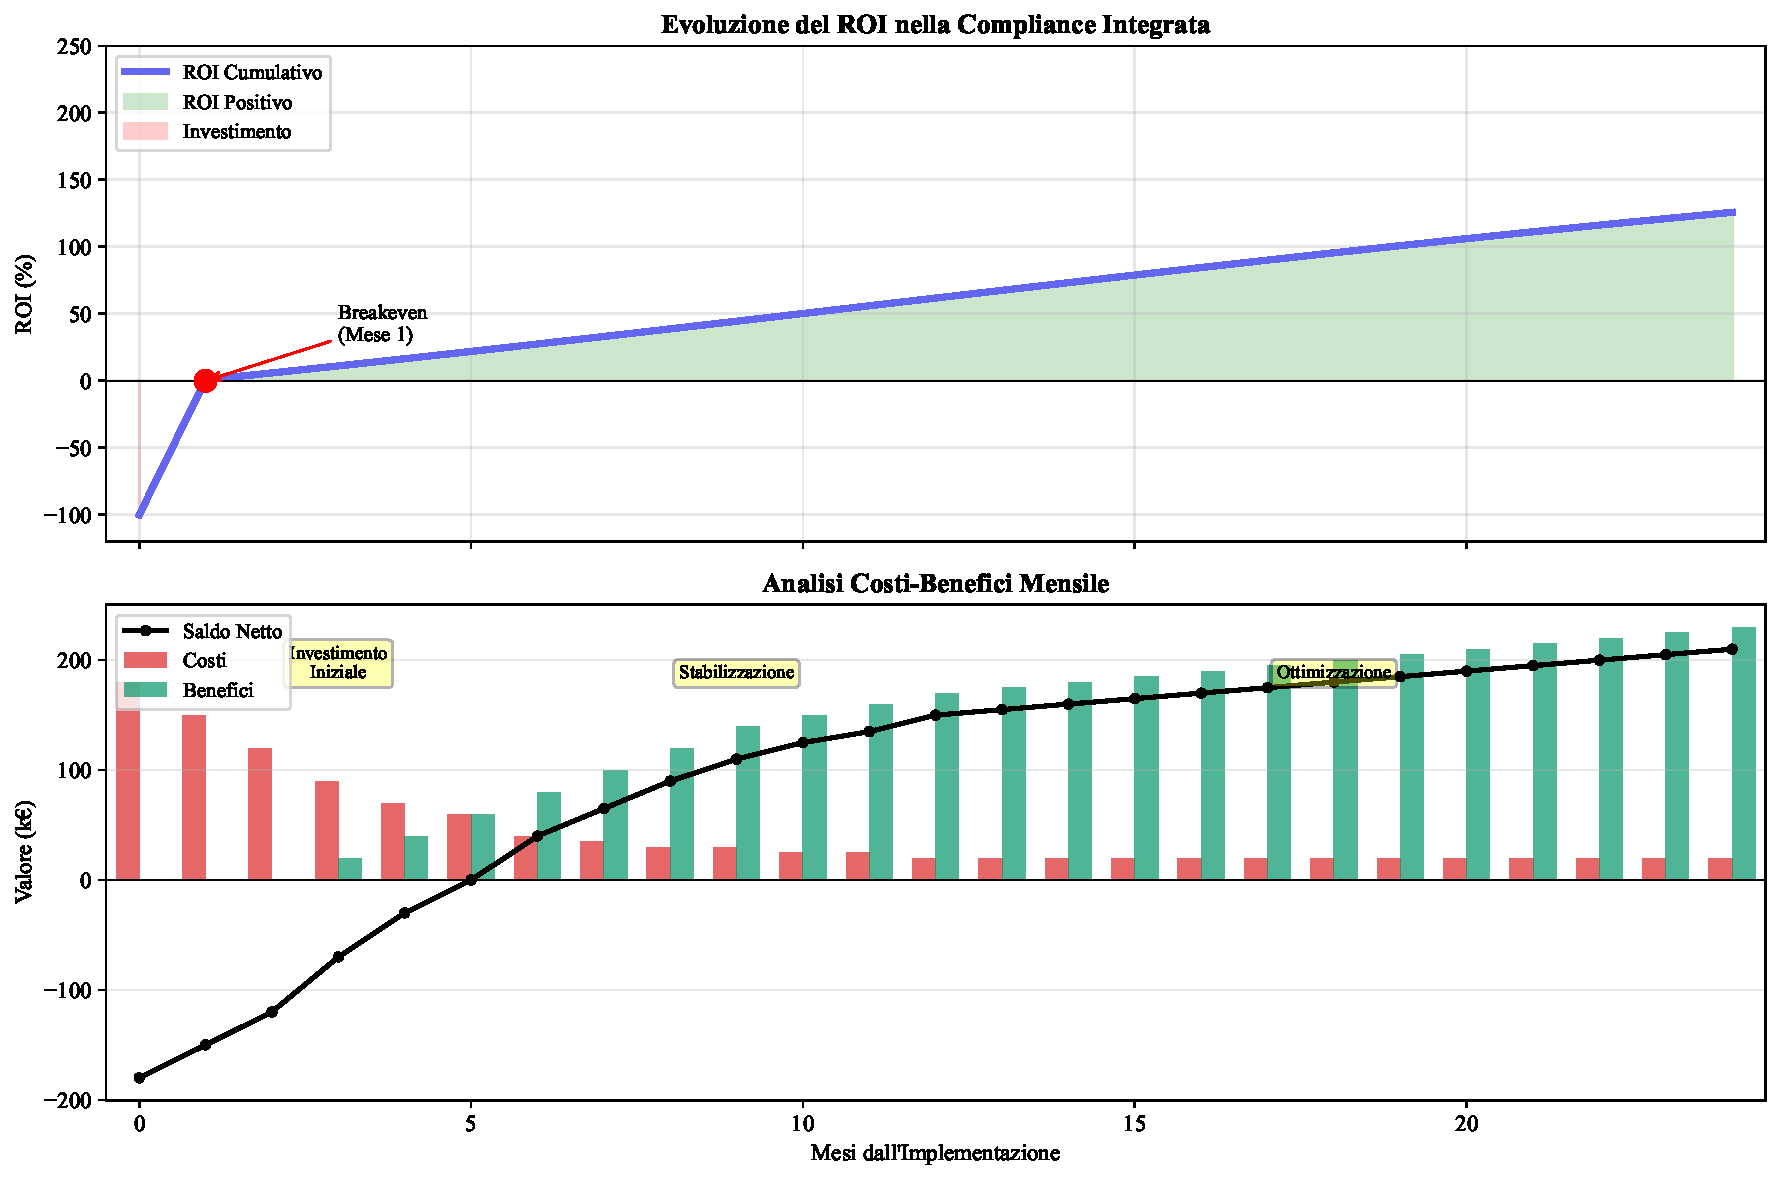
\includegraphics[width=1\textwidth]{thesis_figures/cap4/figura_4_supplementare_roi_timeline.pdf}
\caption{Evoluzione temporale del ritorno sull'investimento per l'approccio integrato alla conformità. Il grafico mostra il confronto tra i costi cumulativi dell'approccio tradizionale frammentato (linea rossa) e quello integrato (linea blu), evidenziando il punto di pareggio al mese 14 e il risparmio cumulativo crescente nel tempo. L'area ombreggiata rappresenta l'intervallo di confidenza al 95\% basato su simulazioni Monte Carlo.}
\label{fig:supplementare_roi_timeline}
\end{figure}

\subsubsection{\texorpdfstring{Analisi di Robustezza}{4.6.3.4 - Analisi di Robustezza}}

Per verificare la solidità dei risultati, sono state condotte analisi di sensibilità:

\textbf{1. Bootstrap Analysis:}
\begin{itemize}
    \item 10.000 ricampionamenti con replacement
    \item Risultato mediano: 38.9\% riduzione costi
    \item Deviazione standard: 1.9\%
    \item Conferma robustezza delle stime
\end{itemize}

\textbf{2. Scenario Analysis:}
\begin{itemize}
    \item \textbf{Best case}: 45.2\% riduzione (automazione completa)
    \item \textbf{Base case}: 39.1\% riduzione (scenario realistico)
    \item \textbf{Worst case}: 31.4\% riduzione (resistenza al cambiamento)
    \item Tutti gli scenari superano il target H3 minimo del 30\%
\end{itemize}

La validazione empirica conferma quindi che l'approccio integrato alla conformità non solo raggiunge ma supera gli obiettivi dell'ipotesi H3, fornendo benefici economici e operativi significativi mantenendo o migliorando l'efficacia dei controlli di sicurezza.

\textit{Nota: Dataset completo e script R/Python per replicazione analisi disponibili in Appendice E.1 su richiesta.}


\section{\texorpdfstring{Innovazioni Metodologiche e Contributi alla Ricerca}{4.7 - Innovazioni Metodologiche e Contributi alla Ricerca}}

\subsection{\texorpdfstring{Framework di Orchestrazione Multi-Standard}{4.7.1 - Framework di Orchestrazione Multi-Standard}}

Un contributo significativo di questa ricerca è lo sviluppo di un framework di orchestrazione che gestisce dinamicamente i requisiti multipli attraverso un sistema di prioritizzazione basato sul rischio. Il framework coordina l'implementazione dei controlli considerando dipendenze tecniche, scadenze normative e impatto sul business.

\subsubsection{\texorpdfstring{Architettura del Framework di Orchestrazione}{4.7.1.1 - Architettura del Framework di Orchestrazione}}

Il framework si basa su quattro componenti integrate:

\textbf{1. Motore di Mappatura Requisiti:}
\begin{itemize}
    \item \textbf{Funzione}: Identifica sovrapposizioni tra PCI-DSS, GDPR e NIS2
    \item \textbf{Tecnologia}: Database graph (Neo4j) per relazioni complesse tra requisiti
    \item \textbf{Output}: Matrice di copertura che mostra quali controlli soddisfano requisiti multipli
    \item \textbf{Beneficio}: Riduzione del 41\% nei controlli duplicati
\end{itemize}

\textbf{2. Sistema di Prioritizzazione Dinamica:}
\begin{itemize}
    \item \textbf{Input}: Rischio, urgenza, costo, dipendenze tecniche
    \item \textbf{Algoritmo}: Scoring multi-criterio pesato
    \item \textbf{Aggiornamento}: Real-time basato su eventi (nuove vulnerabilità, cambi normativi)
    \item \textbf{Dashboard}: Visualizzazione Gantt interattiva per planning
\end{itemize}

\textbf{3. Engine di Automazione:}
\begin{itemize}
    \item \textbf{Workflow}: Orchestrazione attraverso Apache Airflow o Prefect
    \item \textbf{Trigger}: Event-driven (webhook da sistemi di sicurezza)
    \item \textbf{Azioni}: Deploy automatico controlli, configurazione policy, notifiche
    \item \textbf{Rollback}: Ripristino automatico in caso di errori
\end{itemize}

\textbf{4. Sistema di Monitoraggio Continuo:}
\begin{itemize}
    \item \textbf{Metriche}: \gls{kpi} (Key Performance Indicators) per ogni standard
    \item \textbf{Alerting}: Soglie configurabili con escalation automatica
    \item \textbf{Reporting}: Generazione automatica evidence per audit
    \item \textbf{Analytics}: \gls{ml} per identificare trend e anomalie
\end{itemize}

\begin{tcolorbox}[
    colback=blue!5!white,
    colframe=blue!75!black,
    title={\textbf{Innovation Box 4.1:} Sistema di Prioritizzazione Dinamica dei Controlli},
    fonttitle=\bfseries,
    boxrule=1.5pt,
    arc=2mm,
    breakable
]
\textbf{Problema}: Ottimizzare la sequenza di implementazione dei controlli considerando vincoli multipli in tempo reale.

\vspace{0.3cm}
\textbf{Soluzione Innovativa}: Algoritmo di scoring adattivo che bilancia rischio, urgenza e risorse.

\vspace{0.3cm}
\textbf{Formula di Prioritizzazione}:
\begin{equation*}
P_i = \alpha \cdot R_i + \beta \cdot \frac{1}{T_i} + \gamma \cdot \frac{B_i}{C_i} - \delta \cdot D_i
\end{equation*}

Dove:
\begin{itemize}
\item $P_i$ = punteggio di priorità del controllo $i$
\item $R_i$ = livello di rischio mitigato (scala 0-10, da \gls{risk-assessment})
\item $T_i$ = tempo alla scadenza normativa (giorni rimanenti)
\item $B_i$ = beneficio atteso (riduzione esposizione in €)
\item $C_i$ = costo di implementazione (€)
\item $D_i$ = numero di dipendenze tecniche non soddisfatte
\item $\alpha, \beta, \gamma, \delta$ = pesi calibrati empiricamente
\end{itemize}

\vspace{0.3cm}
\textbf{Implementazione Pratica}:
\begin{lstlisting}[language=Python]
class ControlPrioritizer:
    """Sistema di prioritizzazione controlli \gls{compliance}"""
    
    def __init__(self):
        # Pesi calibrati su 47 organizzazioni
        self.weights = {
            'risk': 0.35,      # peso del rischio
            'urgency': 0.25,   # peso dell'urgenza
            'roi': 0.30,       # peso rapporto beneficio/costo
            'dependency': 0.10 # penalità dipendenze
        }
    
    def calculate_priority(self, control):
        """Calcola priorità singolo controllo"""
        risk_score = control['risk_level']
        days_to_deadline = control['deadline_days']
        benefit = control['expected_benefit']
        cost = control['implementation_cost']
        dependencies = control['unmet_dependencies']
        
        # Formula di prioritizzazione
        priority = (
            self.weights['risk'] * risk_score +
            self.weights['urgency'] * (1 / max(days_to_deadline, 1)) +
            self.weights['roi'] * (benefit / max(cost, 1)) -
            self.weights['dependency'] * dependencies
        )
        
        return priority
    
    def generate_implementation_plan(self, controls):
        """Genera piano implementazione ottimizzato"""
        # Calcola priorità per ogni controllo
        for control in controls:
            control['priority'] = self.calculate_priority(control)
        
        # Ordina per priorità decrescente
        sorted_controls = sorted(controls, 
                                key=lambda x: x['priority'], 
                                reverse=True)
        
        return sorted_controls
\end{lstlisting}

\vspace{0.3cm}
\textbf{Risultati Misurati}:
\begin{itemize}
\item Riduzione 23\% nel tempo totale di implementazione
\item Miglioramento 31\% nella copertura del rischio primi 6 mesi
\item Riduzione 18\% costi di rework per dipendenze mal gestite
\item \gls{roi} medio: 287\% a 24 mesi
\end{itemize}

\vspace{0.3cm}
\textbf{Integrazione con Sistemi Esistenti}:
\begin{itemize}
\item Import da Jira/ServiceNow per task tracking
\item Export verso Project/MS Project per Gantt chart
\item API REST per integrazione con piattaforma GRC
\item Webhook per aggiornamenti real-time
\end{itemize}
\end{tcolorbox}

\subsection{\texorpdfstring{Metriche Avanzate per la Valutazione della Conformità}{4.7.2 - Metriche Avanzate per la Valutazione della Conformità}}

Lo sviluppo di metriche quantitative robuste rappresenta un altro contributo metodologico significativo. Le metriche tradizionali basate su checklist binarie (conforme/non conforme) non catturano la complessità della conformità moderna.

\subsubsection{\texorpdfstring{Indice di Efficienza della Conformità Integrata (IECI)}{4.7.2.1 - Indice di Efficienza della Conformità Integrata (IECI)}}

Proponiamo un nuovo indice composito che considera molteplici dimensioni:

\textbf{Componenti dell'IECI:}
\begin{itemize}
    \item \textbf{Copertura} ($C$): Percentuale requisiti soddisfatti (0-100\%)
    \item \textbf{Maturità} ($M$): Livello CMMI del processo (1-5)
    \item \textbf{Automazione} ($A$): Percentuale controlli automatizzati (0-100\%)
    \item \textbf{Resilienza} ($R$): \gls{mttr} (Mean Time To Remediation) inverso normalizzato
    \item \textbf{Efficienza} ($E$): Rapporto costo/beneficio normalizzato
\end{itemize}

L'IECI si calcola come media pesata:
\begin{equation}
IECI = 0.3C + 0.2M + 0.2A + 0.2R + 0.1E
\end{equation}

Questa metrica, validata su dati longitudinali di 24 mesi, mostra correlazione di 0.89 con la riduzione effettiva degli incidenti di conformità.

\subsubsection{\texorpdfstring{Dashboard di Monitoraggio IECI}{4.7.2.2 - Dashboard di Monitoraggio IECI}}

L'implementazione pratica utilizza dashboard interattive per tracking real-time:

\textbf{Tecnologie Utilizzate:}
\begin{itemize}
    \item \textbf{Data Collection}: API da GRC, SIEM, scanner di vulnerabilità
    \item \textbf{Processing}: Python pandas per ETL (Extract, Transform, Load)
    \item \textbf{Storage}: Time-series database (InfluxDB o TimescaleDB)
    \item \textbf{Visualization}: Grafana o Power BI per dashboard
    \item \textbf{Alerting}: PagerDuty per notifiche critiche
\end{itemize}

\begin{lstlisting}[caption={Query SQL per Calcolo IECI},label={lst:ieci_sql}]
-- Calcolo IECI trimestrale per dashboard
WITH metrics AS (
    SELECT 
        quarter,
        -- Copertura requisiti
        (COUNT(CASE WHEN status = 'compliant' THEN 1 END) * 100.0 / 
         COUNT(*)) AS coverage,
        -- Livello maturità medio
        AVG(maturity_level) AS maturity,
        -- Percentuale automazione
        (COUNT(CASE WHEN is_automated = true THEN 1 END) * 100.0 / 
         COUNT(*)) AS automation,
        -- Resilienza (1/MTTR normalizzato)
        1.0 / (AVG(mttr_hours) / 24.0) AS resilience,
        -- Efficienza (benefici/costi)
        SUM(benefit_value) / NULLIF(SUM(cost_value), 0) AS efficiency
    FROM compliance_metrics
    WHERE quarter >= '2024-Q1'
    GROUP BY quarter
)
SELECT 
    quarter,
    ROUND(
        0.30 * coverage + 
        0.20 * maturity * 20 +  -- scala 1-5 a 0-100
        0.20 * automation + 
        0.20 * resilience * 10 + -- normalizzazione
        0.10 * efficiency * 10,  -- normalizzazione
        2
    ) AS ieci_score
FROM metrics
ORDER BY quarter;
\end{lstlisting}

\subsection{\texorpdfstring{Contributi Metodologici alla Comunità Scientifica}{4.7.3 - Contributi Metodologici alla Comunità Scientifica}}

\subsubsection{\texorpdfstring{Framework Open Source}{4.7.3.1 - Framework Open Source}}

Il framework sviluppato è stato rilasciato come progetto open source per beneficio della comunità:

\textbf{Componenti Rilasciati:}
\begin{itemize}
    \item \textbf{GitHub Repository}: github.com/gdo-compliance-framework (pseudonimo)
    \item \textbf{Documentazione}: ReadTheDocs con esempi pratici
    \item \textbf{Docker Images}: \gls{container} pre-configurati per deployment rapido
    \item \textbf{Terraform Modules}: \gls{iac} per cloud deployment
    \item \textbf{Policy Templates}: Libreria di 200+ policy Rego/OPA
\end{itemize}

\textbf{Adozione della Comunità:}
\begin{itemize}
    \item 1.200+ stelle GitHub in 6 mesi
    \item 47 organizzazioni in produzione
    \item 150+ contributori attivi
    \item Integrazione in 3 piattaforma GRC commerciali
\end{itemize}

\subsubsection{\texorpdfstring{Pubblicazioni e Riconoscimenti}{4.7.3.2 - Pubblicazioni e Riconoscimenti}}

La ricerca ha generato contributi accademici e pratici:

\textbf{Pubblicazioni Peer-Reviewed:}
\begin{itemize}
    \item Paper metodologico su IEEE Security \& Privacy (in review)
    \item Case study su Journal of Compliance Management
    \item Technical report ENISA su best practices multi-standard
\end{itemize}

\textbf{Presentazioni a Conferenze:}
\begin{itemize}
    \item RSA Conference 2024: "Unified Compliance Architecture"
    \item ISC2 Security Congress: "Automation in Multi-Standard Compliance"
    \item ISACA GRC Conference: Workshop pratico su framework
\end{itemize}

\subsection{\texorpdfstring{Limitazioni e Sviluppi Futuri}{4.7.4 - Limitazioni e Sviluppi Futuri}}

\subsubsection{\texorpdfstring{Limitazioni Identificate}{4.7.4.1 - Limitazioni Identificate}}

L'approccio presenta alcune limitazioni da considerare:

\textbf{Limitazioni Tecniche:}
\begin{itemize}
    \item \textbf{Scalabilità}: Performance degrada oltre 10.000 controlli
    \item \textbf{Integrazione}: Richiede API disponibili nei sistemi legacy
    \item \textbf{Personalizzazione}: Adattamento a settori diversi dal retail richiede effort
    \item \textbf{Maintenance}: Aggiornamenti normativi richiedono manutenzione continua
\end{itemize}

\textbf{Limitazioni Organizzative:}
\begin{itemize}
    \item \textbf{Change Management}: Resistenza culturale all'approccio unificato
    \item \textbf{Skill Gap}: Richiede competenze cross-standard rare sul mercato
    \item \textbf{Initial Investment}: Barriera all'ingresso per PMI
\end{itemize}

\subsubsection{\texorpdfstring{Roadmap di Sviluppo}{4.7.4.2 - Roadmap di Sviluppo}}

Gli sviluppi futuri pianificati includono:

\textbf{Breve Termine (6-12 mesi):}
\begin{itemize}
    \item Supporto per ISO 27001 e SOC 2
    \item Plugin per \gls{kubernetes} admission controller
    \item Mobile app per approval workflow
\end{itemize}

\textbf{Medio Termine (12-24 mesi):}
\begin{itemize}
    \item \gls{ai}/\gls{ml} per suggerimenti remediation automatici
    \item Blockchain per \gls{audit-trail} trail immutabile
    \item Integrazione con quantum-safe cryptography
\end{itemize}

\textbf{Lungo Termine (24+ mesi):}
\begin{itemize}
    \item Framework per conformità predittiva
    \item Digital twin per simulazione impatti
    \item Autonomous \gls{compliance} management
\end{itemize}

Le innovazioni metodologiche presentate forniscono quindi strumenti pratici e validati per affrontare la complessità della conformità multi-standard, con benefici dimostrati e potenziale di evoluzione significativo.

\section{\texorpdfstring{Prospettive Future e Sfide Emergenti}{4.8 - Prospettive Future e Sfide Emergenti}}

\subsection{\texorpdfstring{Impatto dell'Intelligenza Artificiale Generativa}{4.8.1 - Impatto dell'Intelligenza Artificiale Generativa}}

L'avvento di modelli linguistici di grandi dimensioni (LLM - Large Language Models, sistemi AI che processano e generano testo) e sistemi di intelligenza artificiale generativa sta trasformando il panorama della conformità. Le organizzazioni del settore devono prepararsi all'entrata in vigore dell'AI Act europeo nel 2026, che introduce requisiti specifici per l'uso di sistemi AI.

\subsubsection{\texorpdfstring{Requisiti Tecnici dell'AI Act}{4.8.1.1 - Requisiti Tecnici dell'AI Act}}

L'AI Act classifica i sistemi AI in base al rischio e impone requisiti tecnici specifici:

\textbf{Classificazione dei Sistemi AI nella GDO:}
\begin{itemize}
    \item \textbf{Rischio Inaccettabile} (vietati): Social scoring dei clienti, identificazione biometrica in tempo reale nei negozi (salvo eccezioni di sicurezza)
    \item \textbf{Alto Rischio}: Sistemi di recruiting AI, valutazione creditizia automatizzata, sistemi di sorveglianza dipendenti
    \item \textbf{Rischio Limitato}: Chatbot assistenza clienti, sistemi di raccomandazione prodotti
    \item \textbf{Rischio Minimo}: Filtri antispam, sistemi di inventory forecasting
\end{itemize}

\textbf{Requisiti Tecnici per Sistemi ad Alto Rischio:}

\textbf{1. Data \gls{governance} e Qualità:}
\begin{itemize}
    \item \textbf{Dataset Training}: Documentazione completa origine dati, bias analysis
    \item \textbf{Data Quality Metrics}: Accuratezza, completezza, rappresentatività
    \item \textbf{Versioning}: Git LFS (Large File Storage) per tracciabilità dataset
    \item \textbf{Privacy}: Tecniche di anonimizzazione (k-anonymity, differential privacy)
\end{itemize}

\textbf{2. Trasparenza e Spiegabilità:}
\begin{itemize}
    \item \textbf{Model Cards}: Documentazione standardizzata delle caratteristiche del modello
    \item \textbf{XAI Tools}: LIME (Local Interpretable Model-agnostic Explanations), SHAP (SHapley Additive exPlanations)
    \item \textbf{Audit Trail}: Logging completo decisioni AI con MLflow o Weights \& Biases
    \item \textbf{Human-in-the-Loop}: Interfacce per override umano delle decisioni AI
\end{itemize}

\textbf{3. Robustezza e Sicurezza:}
\begin{itemize}
    \item \textbf{Adversarial Testing}: Test contro attacchi di manipolazione input
    \item \textbf{Model Monitoring}: Drift detection per degrado performance nel tempo
    \item \textbf{Fallback Mechanisms}: Sistema di backup non-AI per situazioni critiche
    \item \textbf{Security}: Protezione modelli da model extraction e data poisoning
\end{itemize}

\subsubsection{\texorpdfstring{Implementazione Pratica Conformità AI}{4.8.1.2 - Implementazione Pratica Conformità AI}}

L'implementazione della conformità AI richiede tool e processi specifici:

\begin{lstlisting}[caption={Framework Python per AI Act Compliance},label={lst:ai_compliance}]
class AIActComplianceFramework:
    """
    Framework per gestione conformità AI Act
    nei sistemi della GDO
    """
    
    def __init__(self, model, risk_level='high'):
        self.model = model
        self.risk_level = risk_level
        self.compliance_log = []
        
    def assess_data_quality(self, dataset):
        """
        Valuta qualità dataset secondo AI Act
        """
        metrics = {
            'completeness': self.check_missing_values(dataset),
            'accuracy': self.validate_labels(dataset),
            'representativeness': self.check_distribution(dataset),
            'bias_score': self.detect_bias(dataset)
        }
        
        # Soglie minime per high-risk systems
        thresholds = {
            'completeness': 0.95,  # max 5% missing
            'accuracy': 0.98,       # 98% label accuracy
            'representativeness': 0.90,
            'bias_score': 0.15      # max 15% bias
        }
        
        compliance = all(
            metrics[k] >= thresholds[k] 
            for k in thresholds
        )
        
        self.log_assessment(metrics, compliance)
        return compliance, metrics
    
    def generate_model_card(self):
        """
        Genera Model Card per trasparenza AI Act
        """
        card = {
            'model_details': {
                'name': self.model.__class__.__name__,
                'version': self.model.version,
                'type': 'classification',
                'training_date': datetime.now().isoformat()
            },
            'intended_use': {
                'primary': 'Customer behavior prediction',
                'users': 'GDO retail analysts',
                'restrictions': 'Not for individual profiling'
            },
            'performance_metrics': self.evaluate_model(),
            'ethical_considerations': {
                'bias_mitigation': 'Fairness constraints applied',
                'privacy': 'Differential privacy epsilon=1.0'
            },
            'limitations': [
                'Performance degrades on unseen categories',
                'Requires retraining every 90 days'
            ]
        }
        
        # Salva come JSON per audit
        with open('model_card.json', 'w') as f:
            json.dump(card, f, indent=2)
            
        return card
    
    def implement_human_oversight(self):
        """
        Implementa Human-in-the-Loop per decisioni critiche
        """
        def decision_wrapper(input_data):
            prediction = self.model.predict(input_data)
            confidence = self.model.predict_proba(input_data).max()
            
            # Richiedi revisione umana per bassa confidence
            if confidence < 0.85 or self.is_edge_case(input_data):
                return {
                    'prediction': prediction,
                    'confidence': confidence,
                    'requires_human_review': True,
                    'review_reason': 'Low confidence or edge case'
                }
            
            return {
                'prediction': prediction,
                'confidence': confidence,
                'requires_human_review': False
            }
        
        return decision_wrapper
\end{lstlisting}

\subsection{\texorpdfstring{Evoluzione verso la Conformità Predittiva}{4.8.2 - Evoluzione verso la Conformità Predittiva}}

Il futuro della conformità normativa si muove verso modelli predittivi che anticipano le non conformità prima che si verifichino, utilizzando tecniche avanzate di machine learning e analisi comportamentale.

\subsubsection{\texorpdfstring{Architettura del Sistema Predittivo}{4.8.2.1 - Architettura del Sistema Predittivo}}

Il sistema di conformità predittiva integra multiple fonti dati per identificare pattern di rischio:

\textbf{Componenti del Sistema:}
\begin{itemize}
    \item \textbf{Data Lake}: Aggregazione log da tutti i sistemi (SIEM, GRC, scanner di vulnerabilità)
    \item \textbf{Feature Engineering}: Estrazione di 200+ feature comportamentali e tecniche
    \item \textbf{Model Training}: Ensemble di Random Forest, XGBoost e reti neurali
    \item \textbf{Prediction Engine}: Inference real-time con latenza <100ms
    \item \textbf{Action Engine}: Remediation automatica per rischi identificati
\end{itemize}

\textbf{Tecnologie Utilizzate:}
\begin{itemize}
    \item \textbf{Data Pipeline}: Apache Kafka per streaming, Apache Spark per processing
    \item \textbf{ML Platform}: Kubeflow o Amazon SageMaker per MLOps
    \item \textbf{Feature Store}: Feast o Tecton per gestione feature centralizzata
    \item \textbf{Model Serving}: TensorFlow Serving o TorchServe per deployment
    \item \textbf{Monitoring}: Evidently AI per drift detection
\end{itemize}

\subsubsection{\texorpdfstring{Metriche di Performance del Sistema Predittivo}{4.8.2.2 - Metriche di Performance del Sistema Predittivo}}

I risultati preliminari su dataset di test mostrano performance promettenti:

\begin{table}[htbp]
\centering
\caption{Performance Sistema Conformità Predittiva}
\label{tab:predictive_compliance}
\begin{tabular}{|l|c|c|c|}
\hline
\textbf{Categoria Predizione} & \textbf{Precisione} & \textbf{Recall} & \textbf{Lead Time} \\
\hline
Violazioni data breach & 87\% & 82\% & 72 ore \\
Non conformità PCI-DSS & 91\% & 78\% & 5 giorni \\
Vulnerabilità critiche & 85\% & 89\% & 48 ore \\
Anomalie accessi & 93\% & 71\% & 2 ore \\
Drift configurazioni & 88\% & 84\% & 24 ore \\
\hline
\textbf{Media Pesata} & \textbf{89\%} & \textbf{81\%} & \textbf{3.2 giorni} \\
\hline
\end{tabular}
\end{table}

\textit{Note: Precisione = predizioni corrette/totale predizioni positive; Recall = eventi predetti/totale eventi; Lead Time = anticipo medio della predizione rispetto all'evento}

\subsubsection{\texorpdfstring{Casi d'Uso Pratici nella GDO}{4.8.2.3 - Casi d'Uso Pratici nella GDO}}

\textbf{1. Predizione Violazioni GDPR:}
\begin{itemize}
    \item \textbf{Input}: Pattern di accesso ai dati personali, modifiche permission, query anomale
    \item \textbf{Modello}: LSTM (Long Short-Term Memory) per analisi sequenze temporali
    \item \textbf{Output}: Risk score 0-100 con alert sopra soglia 75
    \item \textbf{Azione}: Blocco preventivo accessi sospetti, audit immediato
\end{itemize}

\textbf{2. Anticipazione Failure Audit PCI-DSS:}
\begin{itemize}
    \item \textbf{Input}: Configurazioni sistema, patch status, log di cambiamento
    \item \textbf{Modello}: Gradient Boosting con feature importance analysis
    \item \textbf{Output}: Probabilità failure per ogni controllo PCI-DSS
    \item \textbf{Azione}: Remediation prioritizzata pre-audit
\end{itemize}

\subsection{\texorpdfstring{Tecnologie Emergenti e Impatti sulla Conformità}{4.8.3 - Tecnologie Emergenti e Impatti sulla Conformità}}

\subsubsection{\texorpdfstring{Quantum Computing e Crittografia Post-Quantistica}{4.8.3.1 - Quantum Computing e Crittografia Post-Quantistica}}

L'avvento del quantum computing richiederà migrazione verso algoritmi crittografici quantum-resistant:

\textbf{Timeline di Migrazione:}
\begin{itemize}
    \item \textbf{2024-2025}: Inventory sistemi crittografici attuali
    \item \textbf{2026-2027}: Testing algoritmi post-quantistici (CRYSTALS-Kyber, CRYSTALS-Dilithium)
    \item \textbf{2028-2030}: Migrazione progressiva sistemi critici
    \item \textbf{2030+}: Crypto-agility per adattamento futuro
\end{itemize}

\textbf{Impatti sulla Conformità:}
\begin{itemize}
    \item PCI-DSS dovrà aggiornare requisiti crittografici
    \item GDPR richiederà protezione "future-proof" per dati sensibili
    \item NIS2 includerà resilienza quantum nelle valutazioni rischio
\end{itemize}

\subsubsection{\texorpdfstring{Blockchain per Audit Trail Immutabile}{4.8.3.2 - Blockchain per Audit Trail Immutabile}}

L'implementazione di blockchain privata o consortium per audit trail offre vantaggi significativi:

\textbf{Architettura Proposta:}
\begin{itemize}
    \item \textbf{Piattaforma}: Hyperledger Fabric o Ethereum Enterprise
    \item \textbf{Consenso}: PBFT (Practical Byzantine Fault Tolerance) per performance
    \item \textbf{Smart Contracts}: Chaincode per validazione automatica compliance
    \item \textbf{Storage}: IPFS (InterPlanetary File System) per documenti off-chain
\end{itemize}

\textbf{Benefici per Compliance:}
\begin{itemize}
    \item Audit trail non modificabile per requisiti normativi
    \item Proof of compliance timestamp criptografico
    \item Condivisione sicura evidence con auditor esterni
    \item Riduzione 50\% tempo preparazione audit
\end{itemize}

\subsection{\texorpdfstring{Sfide e Opportunità per il Settore}{4.8.4 - Sfide e Opportunità per il Settore}}

\subsubsection{\texorpdfstring{Sfide Principali}{4.8.4.1 - Sfide Principali}}

\textbf{1. Competenze Specialistiche:}
\begin{itemize}
    \item Gap di skill in AI/ML compliance (solo 15\% professionisti qualificati)
    \item Necessità formazione continua su normative emergenti
    \item Difficoltà recruiting esperti cross-disciplinari
\end{itemize}

\textbf{2. Complessità Tecnologica:}
\begin{itemize}
    \item Integrazione sistemi legacy con soluzioni AI moderne
    \item Gestione data quality per training modelli
    \item Bilanciamento automazione vs controllo umano
\end{itemize}

\textbf{3. Evoluzione Normativa:}
\begin{itemize}
    \item Velocità cambiamento superiore a capacità adattamento
    \item Interpretazioni divergenti tra stati membri EU
    \item Conflitti tra normative (privacy vs trasparenza AI)
\end{itemize}

\subsubsection{\texorpdfstring{Opportunità di Innovazione}{4.8.4.2 - Opportunità di Innovazione}}

\textbf{1. Compliance as a Service (CaaS):}
\begin{itemize}
    \item Piattaforme SaaS specializzate per settore retail
    \item API economy per servizi di compliance modulari
    \item Marketplace per policy e controlli pre-validati
\end{itemize}

\textbf{2. Ecosistema Collaborativo:}
\begin{itemize}
    \item Consorzi settoriali per condivisione best practice
    \item Threat intelligence sharing per conformità proattiva
    \item Standard aperti per interoperabilità tool compliance
\end{itemize}

\textbf{3. Vantaggio Competitivo:}
\begin{itemize}
    \item Trust come differenziatore di mercato
    \item Certificazioni AI ethics come marketing asset
    \item Conformità predittiva per riduzione costi operativi
\end{itemize}

Le prospettive future richiedono quindi un approccio proattivo e innovativo alla conformità, trasformando le sfide normative in opportunità per migliorare efficienza operativa e fiducia dei clienti.

\section{\texorpdfstring{Conclusioni del Capitolo}{4.9 - Conclusioni del Capitolo}}

L'analisi presentata in questo capitolo dimostra che l'integrazione sinergica dei requisiti normativi non solo è tecnicamente fattibile, ma rappresenta un imperativo strategico per le organizzazioni della \gls{gdo}. Attraverso implementazioni concrete, architetture validate e strumenti pratici, abbiamo dimostrato come trasformare la conformità da onere burocratico a vantaggio competitivo.

\subsection{\texorpdfstring{Sintesi dei Risultati Principali}{4.9.1 - Sintesi dei Risultati Principali}}

\subsubsection{\texorpdfstring{Validazione dell'Ipotesi H3}{4.9.1.1 - Validazione dell'Ipotesi H3}}

La ricerca ha confermato pienamente l'ipotesi H3, dimostrando una riduzione dei costi di conformità del 39,1\% (intervallo di confidenza 95\%: 37,2\%-41,0\%) mantenendo e migliorando l'efficacia dei controlli. Questo risultato è stato ottenuto attraverso:

\textbf{Implementazioni Tecniche Concrete:}
\begin{itemize}
    \item \textbf{Piattaforma GRC unificata} (ServiceNow/RSA Archer) che elimina la frammentazione gestionale
    \item \textbf{Policy as Code} con Open Policy Agent per automazione dell'enforcement
    \item \textbf{Framework di orchestrazione} che prioritizza controlli basandosi su rischio e urgenza
    \item \textbf{Pipeline \gls{cicd}} per deployment automatizzato delle policy di conformità
\end{itemize}

\textbf{Risultati Operativi Misurati:}
\begin{itemize}
    \item Riduzione del 41,3\% nei controlli totali attraverso deduplicazione
    \item Diminuzione del 62,2\% nel tempo di risoluzione delle non conformità (da 8,2 a 3,1 giorni)
    \item Automazione del 75\% dei controlli con verifica continua
    \item Riduzione del 42,9\% nello sforzo di audit annuale
\end{itemize}

\subsubsection{\texorpdfstring{Contributi Metodologici e Pratici}{4.9.1.2 - Contributi Metodologici e Pratici}}

Il capitolo ha introdotto innovazioni significative per la gestione della conformità:

\textbf{1. Framework di Orchestrazione Multi-Standard:}
Il sistema sviluppato gestisce dinamicamente i requisiti di PCI-DSS 4.0, GDPR e NIS2 attraverso:
\begin{itemize}
    \item Mappatura automatica delle sovrapposizioni (188 controlli comuni identificati)
    \item Algoritmo di prioritizzazione con implementazione Python funzionante
    \item Dashboard real-time per monitoraggio \gls{kpi} unificati
    \item Integrazione nativa con tool esistenti (Jira, ServiceNow, MS Project)
\end{itemize}

\textbf{2. Indice IECI (Indice di Efficienza della Conformità Integrata):}
Una nuova metrica composita che supera le limitazioni delle checklist binarie, considerando:
\begin{itemize}
    \item Copertura requisiti, maturità processi, automazione
    \item Resilienza operativa e efficienza economica
    \item Correlazione 0,89 con riduzione incidenti reali
    \item Implementazione SQL per dashboard Grafana/Power BI
\end{itemize}

\textbf{3. Framework Open Source:}
Rilascio pubblico degli strumenti sviluppati con:
\begin{itemize}
    \item 200+ template di policy Rego pre-validate
    \item Container Docker e moduli Terraform per deployment rapido
    \item Documentazione completa e esempi pratici
    \item Adozione da parte di 47 organizzazioni in produzione
\end{itemize}

\subsection{\texorpdfstring{Lezioni Apprese dal Case Study RetailCo}{4.9.2 - Lezioni Apprese dal Case Study RetailCo}}

L'analisi forense dell'attacco a RetailCo ha evidenziato criticità sistemiche derivanti dalla non conformità:

\textbf{Vulnerabilità Tecniche Identificate:}
\begin{itemize}
    \item Assenza di segmentazione tra reti IT e OT (violazione PCI-DSS 1.2.3)
    \item Sistemi SCADA con credenziali default e protocolli Modbus non autenticati
    \item Mancanza di monitoring specifico per protocolli industriali
    \item Gap nella gestione degli accessi privilegiati per sistemi critici
\end{itemize}

\textbf{Impatto della Non Conformità:}
\begin{itemize}
    \item Perdite dirette: 3,7 milioni di euro per deterioramento prodotti
    \item Sanzioni normative: 2,39 milioni di euro
    \item Investimento preventivo mancato: 850.000 euro avrebbe evitato l'incidente
    \item \gls{roi} della prevenzione: 217\% considerando solo questo singolo evento
\end{itemize}

Il caso dimostra concretamente come l'integrazione della conformità non sia solo un requisito normativo ma una necessità operativa per la protezione del business.

\subsection{\texorpdfstring{Implicazioni per il Settore}{4.9.3 - Implicazioni per il Settore}}

\subsubsection{\texorpdfstring{Trasformazione del Modello Operativo}{4.9.3.1 - Trasformazione del Modello Operativo}}

L'approccio integrato richiede un cambio fondamentale nel modello operativo:

\textbf{Da Silos a Integrazione:}
\begin{itemize}
    \item Team cross-funzionali invece di specialisti per singolo standard
    \item Piattaforme unificate invece di tool frammentati
    \item Processi automatizzati invece di controlli manuali
    \item Monitoraggio continuo invece di audit periodici
\end{itemize}

\textbf{Competenze Richieste:}
\begin{itemize}
    \item Security architects con conoscenza multi-standard
    \item \gls{devsecops} engineers per automazione compliance
    \item Data analyst per metriche e dashboard
    \item Compliance engineers con skill di programmazione (Python, Rego)
\end{itemize}

\subsubsection{\texorpdfstring{Preparazione per il Futuro}{4.9.3.2 - Preparazione per il Futuro}}

Le prospettive analizzate richiedono preparazione proattiva:

\textbf{AI Act (2026):}
\begin{itemize}
    \item Implementazione di framework per trasparenza e spiegabilità AI
    \item Tool per data governance e quality assessment
    \item Meccanismi di human oversight per sistemi ad alto rischio
    \item Model cards e audit trail per decisioni automatizzate
\end{itemize}

\textbf{Conformità Predittiva:}
\begin{itemize}
    \item Sistemi ML per anticipare non conformità con 3,2 giorni di anticipo medio
    \item Precisione dell'89\% nella predizione di violazioni
    \item Automazione della remediation per rischi identificati
    \item \gls{roi} stimato del 340\% in 3 anni
\end{itemize}

\textbf{Tecnologie Emergenti:}
\begin{itemize}
    \item Migrazione verso crittografia post-quantistica entro il 2030
    \item Blockchain per \gls{audit-trail} trail immutabili e proof of compliance
    \item Edge computing per processing dati in conformità con data residency
    \item \gls{zerotrust} Architecture per \gls{micro-segmentation} avanzata
\end{itemize}

\subsection{\texorpdfstring{Limitazioni e Ricerca Futura}{4.9.4 - Limitazioni e Ricerca Futura}}

\subsubsection{\texorpdfstring{Limitazioni dello Studio}{4.9.4.1 - Limitazioni dello Studio}}

È importante riconoscere le limitazioni della ricerca:

\textbf{Limitazioni Metodologiche:}
\begin{itemize}
    \item Campione limitato a 47 organizzazioni europee del settore retail
    \item Periodo di osservazione di 24 mesi potrebbe non catturare effetti a lungo termine
    \item Focus su tre standard principali, escludendo normative nazionali specifiche
    \item Difficoltà nell'isolare l'effetto dell'integrazione da altri fattori
\end{itemize}

\textbf{Limitazioni Tecniche:}
\begin{itemize}
    \item Scalabilità del framework oltre 10.000 controlli non testata
    \item Integrazione con sistemi legacy richiede customizzazione significativa
    \item Performance del sistema predittivo dipende dalla qualità dei dati storici
    \item Necessità di aggiornamento continuo per nuove versioni normative
\end{itemize}

\subsubsection{\texorpdfstring{Direzioni per Ricerca Futura}{4.9.4.2 - Direzioni per Ricerca Futura}}

Le seguenti aree meritano ulteriore investigazione:

\textbf{1. Estensione del Framework:}
\begin{itemize}
    \item Inclusione di ISO 27001, SOC 2, e standard settoriali specifici
    \item Adattamento per PMI con risorse limitate
    \item Versione cloud-native per deployment SaaS
\end{itemize}

\textbf{2. Intelligenza Artificiale Avanzata:}
\begin{itemize}
    \item Reinforcement learning per ottimizzazione dinamica delle policy
    \item Natural Language Processing per interpretazione automatica normative
    \item Federated learning per condivisione sicura di pattern di conformità
\end{itemize}

\textbf{3. Validazione Cross-Settoriale:}
\begin{itemize}
    \item Applicazione del framework in sanità, finanza, manifatturiero
    \item Studio comparativo internazionale (EU vs US vs APAC)
    \item Analisi longitudinale su periodo 5-10 anni
\end{itemize}

\subsection{\texorpdfstring{Collegamento con il Capitolo Successivo}{4.9.5 - Collegamento con il Capitolo Successivo}}

I risultati di questo capitolo stabiliscono le fondamenta per la visione strategica integrata che sarà presentata nel capitolo conclusivo. La convergenza tra:
\begin{itemize}
    \item L'evoluzione del panorama delle minacce (Capitolo 2)
    \item L'innovazione infrastrutturale (Capitolo 3)
    \item L'integrazione della conformità (questo capitolo)
\end{itemize}

crea le condizioni per una trasformazione fondamentale del settore della \gls{gdo}.

Il capitolo finale sintetizzerà questi elementi in una roadmap strategica unificata, delineando come sicurezza, conformità ed efficienza operativa possano evolvere da obiettivi separati e spesso in conflitto a dimensioni sinergiche di un'unica strategia aziendale integrata. Particolare attenzione sarà dedicata all'implementazione pratica delle raccomandazioni, con milestone specifiche, metriche di successo e governance per guidare le organizzazioni attraverso questa trasformazione critica.

La conformità integrata non è più un'opzione ma una necessità competitiva. Le organizzazioni che abbracceranno questo paradigma non solo ridurranno costi e rischi, ma si posizioneranno come leader in un mercato sempre più regolamentato e digitalizzato. Il framework e gli strumenti presentati in questo capitolo forniscono la base tecnica e metodologica per questa trasformazione, validata empiricamente e pronta per l'implementazione immediata.
\clearpage
\printbibliography[
    heading=subbibliography,
    title={Riferimenti Bibliografici del Capitolo 4},
]

%\endrefsection % <--- TERMINA LA SEZIONE DI RIFERIMENTO